\chapter{Spiking Deep Networks}
\chplabel{spike}

%% This chapter of my thesis details how
%% I implemented a deep convolutional neural network
%% using spiking LIF neurons.
%% I will begin by introducing and motivating the problem,
%% and provide background on previous work in the area.

At the end of the previous chapter,
we saw that fixed-encoding networks can be used to construct spiking networks
that perform well on smaller datasets.
However, that method does not generalize well to larger datasets.
Deep artificial neural networks have been used by the machine learning field
to perform object recognition on very large, challenging datasets \parencite{Krizhevsky2012}.
How to construct and train such networks in rate neurons
is a relatively well-studied problem;
how the same types of networks might be constructed and trained
with spiking neurons, less so.
This chapter describes a novel implementation of
a deep convolutional neural network using spiking LIF neurons.
Some of this work has been previously described in
\textcite{Hunsberger2015} and \textcite{Hunsberger2016},
and has been expanded on for this thesis.


\section{Background}

Deep artificial neural networks (DNNs),
specifically convolutional neural networks (CNNs, see \scn{cnns}),
are one of the success stories of modern computer vision.
They have been able to successfully recognize a wide range of objects
in large, complex images \parencite[\eg/][]{Krizhevsky2012}.
However, these networks have all been designed for and run using rate-based neurons.
The question of how they can be run in spiking neurons
is an expanding area of research.

Why would we want to run such networks in spiking neurons?
There are two main motivations behind making deep spiking networks.
The first is to allow some of the large CNN models
that have recently had success at numerous object recognition and other tasks
to run on spiking neuromorphic hardware.
This will open the door for energy-efficient systems
performing object recognition in real time on robotic platforms,
where current technology is too energy-intensive
to allow for deployment on mobile robots, for example.

The second motivation is to bring more brain-like components
into machine learning models.
There are many unique challenges related to learning in the brain,
such as how to deal with the nonlinear nature of neurons,
particularly around their firing thresholds,
and how to deal with the discreteness and variability that comes with
communicating using spikes.
While the spiking deep networks introduced here
are not intended to be models of how the brain learns
(the learning procedure is not neurally plausible),
the challenges addressed in this chapter are also faced by the brain,
and some of the ideas in this part help motivate
the more biologically plausible learning mechanisms proposed
in \chp{learning}.

%% Compared with traditional ANNs, which use real-valued nonlinearities,
%% spiking nonlinearities provide a number of challenges to training the network:
%% \begin{enumerate}
%%   \item Non-differentiability of the nonlinearity
%%   \item Increased variability in the output of the nonlinearity for a fixed input
%%   \item An added dimension of time, resulting in dynamics not observed in traditional ANNs.
%% \end{enumerate}
%% These challenges can and have been addressed in many different ways,
%% with the approaches divisible into two main categories:
%% rate-based methods,
%% which use a firing-rate approximation of the spiking neural process for training;
%% spike-based methods,
%% which typically optimize the spike times of the neurons.

% Differences:
%  - spiking neurons have time
%  - spikes are discrete, and if we look at a time bin the rate is discrete
%  - spiking signal is more ``variable''
Spiking deep networks transmit information between neurons
in the form of discrete spikes.
The first difference to notice about spiking networks is that there
is an added dimension of time not typically present in rate-based DNNs.
That is, a spiking neuron is a process that evolves over time,
sometimes emitting spikes, sometimes not.
It only makes sense to talk about this process over time;
looking at it in one instant tells us little about what is going on.
%% If we discretize time (as is common in numerical simulations of neural processes),
%% then a neuron is either spiking in a time bin, or it is not.
In rate-based networks, on the other hand,
we typically present an input and can instantaneously determine the activities
of each subsequent neuron in the network,
since they do not change over time.

The second difference to notice is that spikes are discrete
and all identical.
The only information that a spike carries is the time at which it occurred.
As discussed in \scn{codes}, this means that there are two main types of codes
a neuron can use: rate codes, or timing codes.
If we use a timing code, then we are concerned about the times of individual spikes.
If we use a rate code, then we are more concerned about the number of spikes
in a particular time window,
or perhaps the relative timing of spikes with respect to one another.
When looking at the number of spikes in a time window,
we are faced with the additional challenge that the resulting rate is discrete.
If there are $n$ spikes in the $t$ second window,
then the firing rate is $n / t$, where $n$ is an integer.
For a fixed window $t$, there are only a discrete number of values that
this firing rate can take on,
specifically all the integer values of $n$.

The third difference to notice is that the output of spiking neurons is
inherently more variable than their rate-based counterparts.
Given a constant input, a rate neuron will give a constant output,
that is, the firing rate corresponding to that input.\footnote{
  Rate neurons can have internal dynamics
  (\eg/ the adapting version of the rate-based LIF),
  and given a constant input, the output of these neurons will not be constant.
  However, their output is still much less variable
  than their spiking counterparts.}
Spiking neurons, on the other hand, will output a spike train,
which when filtered by a synapse,
results in an oscillating signal
whose variability depends on the firing rate.
Thus, even when presented with a constant input,
a spiking network will show variability in the inputs to each neuron,
and the outputs of the entire network.

DNNs are traditionally rate-based,
in that the nonlinearity activity implicitly represents the firing rate of a neuron.
For example, a ReLU can be viewed as a neuron that is silent if its input is below zero,
and whose firing rate increases linearly as the current increases above zero.
Furthermore, rate-based DNNs have cost functions that are based on
the activities (firing rates) of the output neurons:
if the network is performing classification,
the chosen class is the output unit with the highest activity.
One approach is therefore to treat spiking networks similarly,
and train the network so that the unit corresponding to the target class
will have the highest activity.\footnote{
  This activity does not necessarily correspond to a neuron firing rate.
  In fact, it is more likely the filtered, weighted sum over the spiking activities
  of the final layer of neurons in the network.}
The alternative is to train the network so that the first neuron to spike
will be the chosen class.

At the level of a single neuron, this distinction goes away.
The activity of a neuron firing at a regular rate
is captured by its inter-spike interval,
the time between one spike and the next.
Assuming the neuron starts in a resting state,
the inter-spike interval is equivalent
to the time before the first spike of a neuron (plus the refractory period).
The key design decision is how we transmit information between neurons.
\emph{Spike-based optimization methods}
compute the exact spike times of neurons,
and use these to compute the spike times of neurons in subsequent layers.
\emph{Rate-based optimization methods}, on the other hand,
treat neurons as idealized rate-response curves,
and only transmit firing \emph{rates} within the network.

%% The key challenge faced by spiking networks
%% is that there is no clear way to take the derivative of a spiking neuron
%% with respect to its input.
%% The first part of this problem is that it is not even clear
%% what we should take the derivative \emph{of}:
%% should we take the derivative of the firing \emph{rate} of the neuron \wrt/ the input,
%% or should we take the derivative of the first spike \emph{time}?
%% Essentially, this is the question of which metric to use,
%% except here we are talking about a single neuron within the network,
%% not the network output.
%% %% The second part of this problem is that for either choice of metric,
%% %% there is no clear way to take the derivative of the spiking neuron.
%% If we choose the activity metric,
%% then there is no clear way to take the derivative of the spiking neuron.
%% The firing rate of a neuron over a period is a discrete value,
%% since the number of spikes in the interval must be an integer.
%% This means that the derivative is essentially infinite if an infinitesimal
%% change in the input would change the number of output spikes in the interval,
%% and zero otherwise; thus, the derivative is undefined.
%% This is the main challenge faced by \emph{rate-based optimization methods}.
%% If we choose the first-to-spike metric,
%% the procedure for taking the derivative is more clear:
%% if the neuron is currently firing at least one spike,
%% then the derivative is based on how much a change in the input
%% changes the time of that first spike,
%% and if the neuron is not firing a spike,
%% then the derivative is zero
%% (the details vary between implementations).
%% This is the basis for \emph{spike-based optimization methods}.

%% While rate-based and spike-based optimization methods
%% are optimizing different metrics,
%% there is a connection between the activity metric and the first-to-spike metric.
%% Namely, a neuron that spikes more quickly does so because it has stronger inputs,
%% which would also lead to increased activity.
%% It is therefore likely that the networks resulting from these
%% two different optimization methods are quite similar.
%% Their main difference should only be seen
%% when all neural and synaptic activities are starting at zero;
%% in this situation, the first-to-spike metric can better account
%% for the precise timing of spikes and potentially result
%% in a faster decision.
%% Not surprisingly, all the networks I am aware of
%% that use spike-based optimization methods
%% do reset the system between stimulus presentations.
%% Once the networks have been running (for example when using continuous inputs),
%% I expect the two types of networks to perform similarly.
%% However, I am not aware of any such comparison in the literature.


\subsection{Spike-based optimization methods}
\scnlabel{spikingmethods}

Spike-based methods optimize the times of individual neuron spikes
to reduce the overall error of the network.
Because the time at which a neuron spikes is a continuous value,
continuous optimization methods can be used.
However, the problem is still highly nonlinear,
because a small change in the input to a neuron
(and thus a small change to the neuron's input weights)
can push a neuron over its firing threshold,
eliciting a spike and drastically changing the output of the neuron \parencite{Gutig2014}.

%% Typically just care about first spike time, but some relaxing this (Stromatias2014)


%% SpikeProp (Bohte 2000)
The first algorithm to perform supervised deep learning
by optimizing spike times was SpikeProp \parencite{Bohte2002}.
This algorithm makes the simplifying assumption that
each neuron fires at most one spike during the spiking interval,
or if multiple spikes are fired,
only the first is optimized.
It also has the structural qualification that each connection
is composed of many different synaptic terminals,
each with a different synaptic delay and a different connection weight.
They demonstrate that their algorithm can solve the XOR problem,
and performs comparably to backpropagation optimized both
with gradient descent (GD) and Levenberg-Marquardt (LM)
on a number of small datasets
(the largest having 36 input dimensions, six output classes, and 4435 training examples).
The single-spike optimization procedure and multiple connection weights per synapse
have made it difficult to expand this work to larger datasets.
\textcite{McKennoch2006} present two methods to improve
the rate of convergence of SpikeProp,
though the applications are still limited to small datasets.

%% Mostafa2016:
\textcite{Mostafa2016} proposes an alternative to the SpikeProp algorithm,
designed specifically for non-leaky integrate-and-fire neurons.
It relaxes the restriction that a connection must be composed of
many different discrete-delay elements,
and instead uses a more standard network architecture,
with one exponential-synapse connection between each pair of neurons.
They train networks with both one and two hidden layers,
achieving 2.45\% and 2.86\% on MNIST, respectively.
One challenge the author faced was that dropout,
the most common regularization technique,
did not work in the network in question
because it would often prevent neurons from firing at all.
Lacking a good alternative regularization method,
the networks suffered from large generalization errors
(the training error for both networks was almost zero).

%% Stromatias2014: using GA to optimize spike times (allows more than one spike per neuron)
Whereas the previous algorithms only optimize the first spike of each neuron,
\textcite{Stromatias2014} relax this restriction.
They use a genetic algorithm to optimize multiple spikes from each neuron.
However, they only demonstrate their algorithm
on relatively small models with fewer than 10 hidden neurons.
Genetic algorithms often have problems scaling
to problems with many parameters,
thus this algorithm may have trouble scaling to datasets like MNIST or CIFAR-10.

%% Friedeman Zenke (Cosyne DL workshop)

%% Robert Gütig (Cosyne DL workshop)

% --- continuous time methods
% Lee et al (2016) Training Deep Spiking Neural Networks using Backpropagation
% - this is specific to LIF neurons, would not work for adapting (also, deals
%   only with first spike, so definitely not for adapting)

\textcite{Lee2016} also optimize over multiple spikes per neuron.
They ignore the spiking discontinuity during backpropagation,
and treat the output of a neuron as a linear function of its inputs
(where the inputs have been filtered by the membrane of the neuron in question).
This allows them to run the network in spiking neurons during training,
but still perform backpropagation without worrying about discontinuities.
They also ignore the refractory period of the neurons,
stating that it is short compared to the time between spikes
and thus has little effect on firing rates.
They add lateral inhibition components to increase network performance,
but only optimize over the first-order derivatives caused by these connections.
Despite these simplifications,
their method is still able to learn appropriately on the MNIST task,
achieving 1.30\% error using standard SGD
and 1.23\% error using an ADAM optimizer.
While it remains to be seen whether this method
can generalize to larger datasets in a tractable way,
it introduces a number of new ideas for training spiking networks
that will hopefully be improved upon by future work.

\textcite{Huh2017} introduce a novel method
to make the spiking process continuous.
They introduce a gating function $g(V)$ of the membrane voltage $V$
that is greater than zero for voltages near the firing threshold,
and zero otherwise, with unit integral.
They call the region where $g(V) > 0$ the \emph{active zone}.
Rather than having efferent synapses receive a current $\delta(t - t_k)$
when the neuron spikes (crosses the firing threshold) at time $t_k$,
synapses continuously receive current based on $g(V) \diff{V}{t}$.
If the voltage is outside the active zone, this term is zero because $g(V) = 0$.
If the voltage crosses the active zone (and thus the neuron spikes)
the integral of this term is one.
Finally, if the voltage enters the active zone,
but does not cross its upper threshold (\ie/ the firing threshold),
then the integral of the term will be a positive number between zero and one
(this is something akin to a partial spike).
This induced synaptic current is almost identical
to the traditional spiking current $\delta(t - t_k)$ in the extremes
(\ie/ when the neuron is silent or firing reasonably quickly),
but continuous in the middle region.
The authors can then achieve a gradient through the network
at any particular point in time using backpropagation,
and optimize the entire network using backpropagation through time.
Their results focus on tasks that require dynamic, temporal representation,
such as predictive coding.
This is a different focus than most other spike-based methods,
which typically focus on static tasks (\ie/ object classification),
and thus a direct comparison is difficult.
Because the method makes the neural nonlinearity differentiable,
it allows the use of many different neuron models:
the paper uses non-leaky integrate-and-fire and
quadratic integrate-and-fire,
and others would certainly be compatible.
This, along with the ability to optimize recurrent spiking networks well,
make this a potentially powerful method for dynamic spiking networks.
For networks focused on static tasks,
I believe that the requirement of this method to optimize over
potentially long time series for each input stimulus
would make it ill-suited for training large object classification networks.

To date, spike-based optimization methods have not been applied
to larger, deeper architectures like CNNs.
This has prevented spike-based training on any datasets
larger or more challenging than MNIST.
Part of the challenge is simply computational:
spike-based optimization methods require more computational resources
than rate-based methods,
since the network is dynamic and requires iterative simulation
for each stimulus presentation.
Most of the current software has been designed for static ANNs,
and expanding it to spiking networks is non-trivial.
%% The other part of the challenge is that convolutional networks use tied weights.
%% While most spike-based algorithms do generate a gradient,
%% and the gradient for a tied weight is simply the sum of the individual gradients
%% across the equivalent untied components,
%% it is not yet tested how well this will work in spiking networks,
%% since it will limit the control over
%% For these reasons,
For this reason,
researchers have turned to rate-based optimization methods
to tackle larger datasets with spiking networks;
this is the focus of the next section.


\subsection{Rate-based optimization methods}
\scnlabel{ratemethods}

Rate-based optimization methods make the simplifying assumption
that all neurons are performing rate coding (see \scn{codes}).
Therefore, these methods do not care about the times of individual spikes,
only the number of spikes over a time period.
Almost always, these types of methods use this simplifying assumption
to replace the spiking neural process with a continuous-valued rate approximation.
For derivative-based methods, this rate approximation is then differentiated.
Derivative-free methods, on the other hand, avoid taking the derivative
of this rate approximation,
and instead opt for an optimization method such as Contrastive Divergence
that does not require it.
Finally, function approximation methods approach the problem differently:
rather than assuming a network of spiking neurons and trying to find
rate approximations to these spiking neurons,
they choose an arbitrary nonlinearity for training the network,
and then use spiking neurons to approximate this nonlinearity.


\subsubsection{Derivative-based methods}

\textcite{Perez-Carrasco2010} describe the first work to train a spiking convolutional network.
%% and one of the first examples of a
They trained a traditional CNN with tanh units using backpropagation.
To convert this to a spiking network,
they replaced the tanh units with binary threshold units
with a refractory period.
Specifically, if the input to a neuron is above a certain threshold,
it fires a spike,
after which the neuron cannot spike for a set period.
This refractory period causes the firing rates of the neurons to saturate.
The authors argue that this helps to ``emulate the corresponding sigmoid functions''
(that is, the tanh function) used in the rate model.
They do not explain exactly how the refractory period does this.
Presumably, they mean because the tanh function is a saturating nonlinearity,
having the neuron firing rate saturate makes the firing rate curve
more similar to the tanh curve.

%% then converted this to a spiking network by approximating the tanh units
%% with IF units with refractory period.
%% The refractory period causes the spike rate to saturate,
%% allowing the unit to better fit the tanh curve.

\textcite{Cao2014} took a more principled approach to converting
rate-based CNNs to spiking CNNs.
They took advantage of the fact that rectified linear units (ReLUs)
perfectly model the rate of a non-leaky integrate-and-fire neuron (IF).
Since ReLUs are currently the standard for deep networks,
this allows networks to be trained with the same rate-based ReLUs,
and then replaced with spiking IF neurons at runtime.
They also replaced the max-pooling layers used by the network
with average pooling layers.
Average pooling layers only involve summing and scaling the inputs,
allowing them to work well with spiking neurons,
moreover in a biologically plausible manner.
Max pooling, on the other hand, has no clear spiking analogue:
taking the max of the binary spikes coming in at the current point in time
(\ie/ outputting one if any of the inputs are spiking, and zero otherwise)
is not at all equivalent to taking the max across spike \emph{rates},
as performed by traditional CNNs.
Furthermore, even taking the max across spikes is not biologically plausible,
since there is no clear neuron-level mechanism for taking the max
across incoming signals.
\textcite{Cao2014} also removed biases from the network,
since they felt these would be difficult for a spiking network to implement.
However, it is not clear why biases would present a problem for spiking networks,
particularly if targeting neuromorphic hardware (much of which supports biases).
%% and later works have included biases.
One advantage to removing biases is that it presents a slightly cleaner biological explanation,
since the output of each neuron depends only on the inputs from other neurons in the network.

\textcite{Diehl2015} employed a similar method to \textcite{Cao2014},
with the addition of a novel normalization method for weight magnitudes.
One key design decision in spiking networks is the tradeoff between
the firing rates of the neurons
and the amount of time needed by the network to make a decision (integration time).
Higher firing rates allow the network to transmit information more quickly,
resulting in faster responses and higher accuracy,
but also use more energy,
and on some neuromorphic platforms there are maximum allowable firing rates.
Increased integration time allows more information to be collected,
resulting in higher accuracy,
but also leads to slower responses and more spikes per example.
Thus, to achieve a balance between
accuracy, response time, and energy efficiency,
the firing rates and integration time need to be properly tuned.
Because ReLUs---and by extension IF neurons---are scale invariant,
the firing rates of neurons in spiking IF networks can be arbitrarily set.
To change the firing rate of a neuron while maintaining the same network,
an increase in the firing rate of the neuron must be met with
a decrease in all connection weights emanating from that neuron.
\textcite{Diehl2015} presents two techniques to normalize network weights
using these ideas: model-based normalization; and data-based normalization.
Both methods are based around the criterion that we do not want
the input to any neuron in a single timestep to be greater than
the firing threshold of that neuron.
If that were to happen,
it could cause the neuron to need to fire two spikes in the same timestep,
something that is not supported by most neuromorphic hardware.
In other terms,
the goal of the normalization is to ensure the instantaneous firing rates
of all neurons never exceeds the rate of the neuromorphic chip (simulation rate).
Model-based normalization finds the maximum sum of positive input weights
across all neurons in a layer,
and then normalizes all neuron inputs in the layer using this sum.
This ensures that no neuron could receive an input greater than
one (the firing threshold) in a single timestep.
The authors found that this technique can make the weights smaller than necessary,
since the maximum possible input to a neuron is often never encountered in real data,
resulting in longer-than-necessary integration times.
Data-based normalization instead bases the normalization
on the examples in the training data.
It ensures that for any given training example,
no neuron will receive an input greater than one (the firing threshold).
The authors found that data-based normalization
decreased the amount of integration time needed by the network
to achieve the same accuracy,
as compared with an un-normalized network with higher firing threshold.
This paper presented state-of-the-art results for spiking networks
on the MNIST dataset, achieving 0.88\% test-set error.

\textcite{Esser2016} trained deep networks
targeting the IBM TrueNorth neuromorphic chip \parencite{Merolla2014}.
Unlike the other networks described here,
this network uses a simple binary threshold neuron,
which fires a ``spike'' if its input is positive at a given time step,
otherwise it is silent.
This is equivalent to a rate-based binary threshold unit.
Additionally, the network only presents each image for a single timestep
before resetting all neuron voltages and presenting the next image.
These considerations make the network rate-based, rather than spiking.
%% Since this neuron function is not differentiable
%% (the derivative is zero at $x = \infty$ and zero elsewhere),
%% they approximated the derivative with the function $\max(0, 1 - \|x\|)$.
They trained very large networks (8 million neurons)
on a number of tasks (including CIFAR-10 and SVHN).
Their results are state-of-the-art if compared to spiking networks,
but the better comparison is to rate-based networks,
where the only innovation is the use of binary threshold units,
which are not commonly used in deep networks.
The network is able to run on neuromorphic hardware (TrueNorth),
but uses many neurons even for modest datasets like CIFAR-10,
and would be difficult to scale to large datasets like ImageNet.


\subsubsection{Derivative-free methods}

Derivative-free, rate-based optimization methods
use rate approximations for the spiking neural process,
but do not require the derivative of the rate approximation.
All such methods I have found base their work on
using the Contrastive Divergence (CD) algorithm \parencite{Hinton2006a}
to train deep networks of stacked RBMs.

\textcite{OConnor2013} create a spiking network of LIF neurons using RBMs.
For training the network,
they use the Siegert approximation to a noisy spiking LIF neuron
as the rate neuron model.
The Siegert approximation is an equation for the mean firing rate of an LIF neuron
given many input spike trains,
where spikes are Poisson distributed with constant firing rate.
These output rates are then normalized by the maximum firing rate $1/t_\text{ref}$
to generate firing probabilities,
and the hidden units are sampled from a binary distribution based on these probabilities.
Training with this model allows the authors to
model some of the variability caused by using spikes.
%% Surprisingly, when running the spiking network for inference,
%% the authors use the Siegert approximation again to determine firing rates
%% and then
They then substitute spiking LIF neurons for these rate neurons
and run the network using Poisson input trains based on pixel intensities,
achieving 5.91\% error on MNIST.
\textcite{Stromatias2015} extends this work by showing that the method
is robust to reduced weight precision,
achieving lower error (5.06\%) on MNIST
using only 11-bit fixed point weights\footnote{
  The 11-bit weights use 3 bits for the integer component
  and 8 bits for the fractional component.}
running on the SpiNNaker platform.

\textcite{Neftci2013} also develop spiking RBMs using LIF neurons.
Their approach fits the average firing rate of a noisy LIF neuron
to a sigmoid curve,
and then trains using this sigmoid curve.
This limits the choice of parameters for the LIF neuron,
in that they must allow the firing rate to be accurately fit by a sigmoid;
however, it allows the RBMs to be trained with traditional sigmoid activation functions,
making the training simpler and more efficient.
They propose an online variant of CD for spiking networks,
building off of an STDP learning rule.
For each presented training image, there are two phases.
The first occurs immediately when the image is presented,
and updates connections based on the data (stimulus).
Then, after a period of time, the recurrent connections become active,
driving the network towards its reconstruction distribution;
this has an effect similar to Gibbs sampling in the CD algorithm.
During this time, the gating signal on the derivative is flipped,
such that the weights are affected negatively based on the reconstruction.
This forms one complete cycle of the algorithm,
and is repeated on each training image,
for many iterations through the training data;
this has an overall effect similar to CD,
thus the authors call it ``event-based CD''.
Using this method, they achieve 8.1\% test-set error on MNIST in spiking neurons.


\subsubsection{Function approximation methods}

Function approximation methods are significantly different than
the previously introduced methods.
Rather than using one spiking neuron to replace each node in the ANN,
function approximation methods use multiple spiking neurons for each node.
They use these spiking neurons to approximate the nonlinear function
(\eg/ sigmoid function) being computed by the node.

I am only aware of one such use of this method, by \textcite{Eliasmith2012}.
They use three spiking LIF neurons to approximate the sigmoid function
computed by each node.
They choose random parameters for each neuron;
most significantly,
they assign a uniformly-distributed random bias current to each neuron.
This allows each of the three neurons to target a different portion of
the sigmoid curve,
and is in addition to the bias current for the node
which is set when training the network.
Once these random parameters are set,
they solve for a scalar weighting for each neuron
that determines how much it contributes to the sigmoid function.
This is the standard NEF method for function approximation (see \scn{nef}),
but applied on a small pool of neurons to approximate a sigmoid function.

This method allows a spiking network to approximate a rate-based network
in a very general way.
One disadvantage is that it uses many more neurons than nodes in the network,
making it more costly in terms of neural resources
than the methods described above.
Its effectiveness also depends highly on how well the neurons can represent
the node function in the operational domain.
Sigmoid functions are relatively easy to represent with LIF neurons.
ReLUs are much flatter and are not squashing,
meaning that the range of output values that the LIF neurons
need to accurately represent is much larger;
this makes them much less amenable to this method.
%% The choice of parameters


\subsection{Noise}

Transmitting discrete, constant-amplitude spikes
(as done throughout much of the human central nervous system)
is a higher-variance method of information transmission
than simply sending a scalar value (such as a voltage).
When taking a rate-based view of neural activity,
one can view this increased variance as ``noise''
around the firing rate (which is the ``signal'').
The firing rate corresponds to the mean value of a spike train signal.
If we pass a spike train through a low-pass filter,
we can view the result as an estimate of this mean
with some additional time-varying noise around it.
The amount of noise depends on the filter used;
cutting out more of the high frequencies
will result in a better estimate with less noise,
but if the underlying firing rate signal is also time-varying,
then we will cut out its higher frequencies as well.
For a spiking network that is receiving a sequence of images
and outputting a response for each in real-time,
this amounts to a longer response time for each image.

Many rate-based spiking neural networks
do not model the variance caused by spikes.
Of those that do, there are two approaches that have been used.
The first is to model the effects of spike noise on the mean neural firing rates,
and then use these revised mean rates when training the model.
The second approach is to include stochastic elements in the model during training,
so that the probability distribution of the training output rates models,
in some way, the variance caused by the spikes used during testing.

%% O'Connor 2013 accounts for spike noise with Siegert model
An example of this first approach is using the Siegert model
to account for the effects of incoming spikes on the LIF neuron firing rate,
as done by \textcite{OConnor2013}.
This approach assumes that neuron inputs are uncorrelated,
with spikes governed by a Poisson process.
The Siegert model then gives the average firing rate of the LIF neuron,
given the average firing rates of all inputs and their respective connection weights.
One drawback to this approach is that the Siegert equation is complicated:
it contains an integral with no closed form solution,
whose integrand contains both the exponential and error (\textrm{erf}) functions.
Computing this function on a GPU (or even a CPU) would be difficult and time-consuming
compared with the functions normally used in neural networks.
The other drawback of this approach is that it requires computing
two linear functions of the input neuron rates,
one to compute the overall input mean and the other to compute the variance.
This means that it requires twice as many matrix-vector operations
as the same network without the Siegert model.

%% Discrete sampling noise: \eg/ Boltzmann machines
%% Noise in RBMs: Nair and Hinton 2010?
The second approach---adding stochastic elements to model spiking noise---%
has often been used in various types of neural networks,
though not with the intent of running the final model in spiking neurons.
A foundational example is Boltzmann machines,
which use binary sampling on probabilistic units \parencite{Hinton1983}.
This allows units to only communicate binary values with one another,
which shares some similarity with spikes.
However, if one views each unit as wanting to transmit
its underlying firing probability (which is like a firing rate),
then this is a very severe form of noise.
Subsequent work by \parencite{Nair2010} greatly relaxed the amount of noise
by having units use rectified linear activation functions
with Gaussian noise on the neuron input.
%% Having such noise sources in a model essentially regularizes the model
Another example of adding stochasticity to a model
is denoising autoencoders \parencite{Vincent2008},
which add noise to model inputs and then attempt
to reproduce the noise-free version of the input.
Adding noise to model inputs has often been used
to help make models better able to deal with a variety of inputs,
essentially it is a type of data augmentation.\footnote{
  Other forms of data augmentation,
  such as translating, rotating, or deforming images,
  can also be viewed as noise on model inputs,
  albeit a more structured form of noise than Gaussian noise.}
However, adding noise to hidden units---%
whether that be to their inputs or outputs---%
is much less common in nonlinear networks \parencite{Poole2014}.
I could not find any examples of it being used
to model the variability caused by spikes
in order to transfer a rate model into spiking neurons.

% Bishop1995: Training with Noise is Equivalent to Tikhonov Regularization


%%%%%%%%%%%%%%%%%%%%%%%%%%%%%%%%%%%%%%%%%%%%%%%%%%%%%%%%%%%%%%%%%%%%%%%%%%%%%%%%
\section{Implementation}

The previous section outlines the many types of methods available
for training deep spiking networks;
each approach has advantages and disadvantages,
with no clear preferred method.
My goal was to implement a deep spiking network
that could process real-world-sized images
depicting a large variety of object categories.
Ultimately, I wanted something that would be able to
process the ImageNet dataset,
a much larger dataset than any spiking network had previously processed.

The ImageNet dataset has a number of defining characteristics:
the images are quite large ($256 \times 256$),
there are over a million training images,
and they are difficult to categorize.
Because of the size, I needed a method that could quickly process
many large images.
This immediately suggested spike-based optimization methods
would not be a good choice,
since they require running each image for a period of time to generate spikes.
If each image needs to run for 100 timesteps,
this means that such dynamic methods would take 100 times longer
than comparable static methods
(assuming no specialized hardware for accelerating spiking computations).
Additionally, all networks that have been successful on ImageNet
are rate based, and by expanding on these methods
I could make use of existing code for training them.

Within the rate-based methods,
I had a choice between derivative-based and derivative-free methods.
The derivative-free methods that I found were all based on
unsupervised learning techniques,
whereas all networks that are successful on the ImageNet dataset
have been trained in a highly supervised manner.
Finally, I did not pursue function approximation methods in depth
because they require many more neurons than methods that incorporate
the neuron tuning curves directly.
Also, my preliminary investigation into function approximation methods
showed that it is difficult to use spiking LIF neurons to properly
represent a ReLU function,
because ReLUs are non-squashing and thus have a wide range of outputs.

These reasons pushed me to implement a deep spiking network
using a derivative-based rate method,
specifically by training a rate-based ANN with neuron-like nonlinearities,
then converting this to a spiking network.
This required three main steps, which I will describe in detail in this section:
1) modifying the architecture to remove components difficult
to implement in neurons;
2) designing a nonlinearity similar to the LIF neuron, but differentiable;
and 3) adding noise during training to increase robustness to spiking variability.
The trained network is then tested with dynamic, spiking neurons.
Since these neurons output signals (\ie/ spike trains)
rather than static scalar values,
the classification procedure also needs to operate over time (see \scn{nef-spiking-methods}).

I evaluate the system on five different datasets:
MNIST, SVHN, CIFAR-10, CIFAR-100, and ILSVRC-2012 (ImageNet).
The datasets are presented in detail in \scn{datasets}.


\subsection{Architecture and modifications}
\scnlabel{spike-architecture}

I based my architecture off of AlexNet \textcite{Krizhevsky2012}.
This architecture won the ILSVRC-2012 (ImageNet) competition,
and a smaller variant of the network achieved $\sim$11\% error on the CIFAR-10 dataset.
I chose it because it is relatively simple,
with very efficient training code freely available.\footnote{
  \url{https://github.com/akrizhevsky/cuda-convnet2}}
%% The AlexNet architecture, though no longer state of the art,

\begin{table}
  \centering
  \begin{tabular}{cc}
    AlexNet & My model \\\hline\hline
    input, 3 channels, $224 \times 224$ & input, 3 channels, $224 \times 224$ \\\hline
    conv 64, size 11, stride 4, padding 0 & conv 64, size 11, stride 4, padding 0 \\
    \textbf{cross-map norm, size 5} & \\
    \textbf{max} pool, size 3, stride 2 & \textbf{avg} pool, size 3, stride 2 \\\hline
    conv 192, size 5, stride 1, padding 2 & conv 192, size 5, stride 1, padding 2 \\
    \textbf{cross-map norm, size 5} & \\
    \textbf{max} pool, size 3, stride 2 & \textbf{avg} pool, size 3, stride 2 \\\hline
    conv 384, size 3, stride 1, padding 1 & conv 384, size 3, stride 1, padding 1 \\
    conv 256, size 3, stride 1, padding 1 & conv 256, size 3, stride 1, padding 1 \\
    conv 256, size 3, stride 1, padding 1 & conv 256, size 3, stride 1, padding 1 \\
    \textbf{max} pool, size 3, stride 2 & \textbf{avg} pool, size 3, stride 2 \\\hline
    full 4096 & full 4096 \\
    dropout, keep 0.5 & dropout, keep 0.5 \\
    full 4096 & full 4096 \\
    dropout, keep 0.5 & dropout, keep 0.5 \\
    full 1000 & full 1000 \\
    \textbf{softmax} & \textbf{softmax (train only)} \\
  \end{tabular}
  \captionb{Details of the AlexNet architecture and the modified version used here.}{
    This is the architecture used for the ImageNet ILSVRC-2012 dataset.
    Differences are highlighted in bold.
    ``conv $n$'' refers to a convolutional layer with $n$ feature maps,
    where ``size'' specifies the filter size.
    ``cross-map norm'' refers to a cross-map normalization layer,
    where ``size'' is the $s$ parameter of the layer.
    ``max pool'' is a max-pooling layer, and ``avg pool'' is an average pooling layer.
    ``full $n$'' is a fully-connected layer with $n$ output neurons.
    ``dropout'' is a dropout layer,
    where ``keep'' is the fraction of output units to keep.
  }
  \tablabel{architectures}
\end{table}

The network is a CNN,
and makes use of the core components of CNNs outlined in \scn{cnns}.
The details of the original architecture are given in \tab{architectures},
along with my modified architecture.\footnote{
  This is the architecture used for the ImageNet ILSVRC-2012 dataset.
  For the other datasets tested,
  I used simplified versions of the architecture.
  Details of these architectures,
  along with all the code for running them,
  can be found at \url{http://github.com/hunse/cuda-convnet2}.}
The original architecture begins with two \emph{generalized convolutional layers},
where each such layer consists of a convolutional layer,
a normalization layer, and a pooling layer.
These are followed by three convolutional layers,
with one pooling layer at the end.
These convolutional layers do not change the size of the image,
and having three of them allows the network to compute more complex nonlinearities.
These are followed by two fully-connected layers, each with dropout.
Finally, the classifier consists of a fully-connected layer
mapping to the 1000-class output space, with a softmax layer.
Neural nonlinearities always occur after each weight layer,
that is, each convolutional or fully-connected layer.
The only exception is the final layer,
where the softmax nonlinearity takes the place of the neural nonlinearities.
Training is performed using a modified version of the LIF rate response function,
described in \scn{softlif}.
For testing, I then run the network dynamically using spiking LIF neurons.

To facilitate running this architecture with spiking neurons,
I made two main modifications.
The first was to remove the normalization layers.
Though normalization layers take inspiration from biology \textcite{Jarrett2009},
it is not clear how spiking neurons could efficiently and robustly
perform this computation.
This type of computation would likely require lateral connections between neurons,
making the network recurrent, and no longer feedforward.
Recurrent networks are much more difficult to train than feedforward ones,
and would require completely different training methods.
As we will see, the normalization layers are non-essential,
and by removing them I was able to train the spiking network using the same
feedforward methods as used on the original network.

The second modification I made was to replace
the max-pooling layers with average-pooling layers.
Like normalization, the ``max'' function is a nonlinear function
that is difficult to compute using spiking neurons.
Again, one way to implement something similar would be with lateral connections,
but I avoided these for the reasons stated above.
Average-pooling, by comparison,
is easy to compute in spiking neurons, since it is a linear operation.

The final structural modification was to use the final softmax layer
during training only,
thereby avoiding the need to implement a ``softmax'' function using spiking neurons.
However, since the classification method takes the maximum output of the network,
and the ``softmax'' function does not affect the maximum value,
this modification should have no effect on the system output.

\begin{table}
  \centering
  \begin{tabular}{lrrrr}
    Dataset & \# neurons & \# weights & \# synapses & FLOPs \\\hline
    MNIST & 27 088 & 6 318 000 & 11 623 200 & 23 298 576 \\
    SVHN & 27 088 & 6 318 800 & 12 250 400 & 24 552 976 \\
    CIFAR-10 & 49 536 & 2 109 376 & 19 512 576 & 39 120 768 \\
    CIFAR-100 & 49 536 & 2 213 056 & 19 616 256 & 39 328 128 \\
    ILSVRC-2012 & 493 184 & 61 090 496 & 714 188 480 & 1 429 246 976 \\
  \end{tabular}
  \captionb{Size metrics for the networks used on all the different tasks.}{
    The number of parameters in each model is equal to the number of weights
    plus the number of neurons (to account for each neuron's bias).
    For fully-connected or locally-connected layers,
    the number of synapses is equal to the number of weights,
    since each weight corresponds to one connection.
    In convolutional layers, the same weight is used for many neural connections;
    this is why the number of synapses is much greater than the number of weights.
    The floating-point operations (FLOPs) corresponds
    to the number of operations required to run the network
    as an ANN using rectified-linear units.
    This will provide a point of comparison
    for running the networks on neuromorphic hardware,
    examined in \scn{spike-efficiency}.
  }
  \tablabel{network-sizes}
\end{table}

A summary of the sizes of the architectures used for each of the tasks
is given in \tab{network-sizes}.
It also presents the number of floating point operations (FLOPs)
required to process one image using the ANN version of the network.
The network used for the ImageNet ILSVRC-2012 task
has ten times more neurons and parameters
and takes 36 times as many FLOPs per image
as any of the other networks.
%% An e


\subsection{The soft-LIF rate neuron}
\scnlabel{softlif}

As described in \scn{ratemethods},
a number of previous works have run deep spiking neuron models
using non-leaky integrate-and-fire (IF) models
without any refractory period between spikes.
This model is particularly amenable to use in spiking deep networks
because its rate response function
is equivalent to the rectified linear unit (ReLU) function
that has become ubiquitous in deep networks.

In my model, I use a \emph{leaky} integrate-and-fire (LIF) neuron model
with a refractory period between spikes.
This not only adds biological realism,
but the refractory period limits the maximum firing rate of the neurons,
potentially reducing their average firing rates as well
and thereby making the networks more efficient on neuromorphic hardware.
However, the LIF neuron model has an added restriction
as compared with the IF model:
Its rate response function is not differentiable.
Specifically, the derivative of the spike rate of an LIF neuron
goes to infinity at the firing threshold.
This unbounded derivative creates numerical problems
for algorithms that require the derivative of the nonlinearity.

To address this, I develop a smoothed (``soft''),
differentiable version of the LIF rate response curve.
This smooth nonlinearity can be used for training a deep neural network,
and then these same parameters can be used to run a spiking version of the network.
The smoothing is adjustable such that the soft-LIF curve can be made
arbitrary close to the LIF rate response curve.

The rate response function for the normalized LIF neuron
is given by \eqn{lifrate}.
We can re-write this equation:
\begin{align}
  r(j) &= \left[\tref - \taurc \log\left(1 - \frac{1}{j}\right)\right]^{-1} \nonumber\\
       &= \left[\tref - \taurc \log\left(\frac{j - 1}{j}\right)\right]^{-1} \nonumber\\
       &= \left[\tref + \taurc \log\left(\frac{j}{j - 1}\right)\right]^{-1} \nonumber\\
       &= \left[\tref + \taurc \log\left(1 + \frac{1}{j - 1}\right)\right]^{-1} \nonumber
\end{align}
if $j > 1$, and zero otherwise.
Since $r = 0$ if $j = 1$, then we can re-write the equation as
%% so that $j - 1 = 0$ if $j \leq 1$:
\begin{align}
  r(j) &= \left[\tref + \taurc \log\left(1 + \frac{1}{\rho(j - 1)}\right)\right]^{-1} \text{ ,}
  \eqnlabel{lifraterho}
\end{align}
where $\rho(x) = \max(x, 0)$.

\begin{figure}
  \centering
  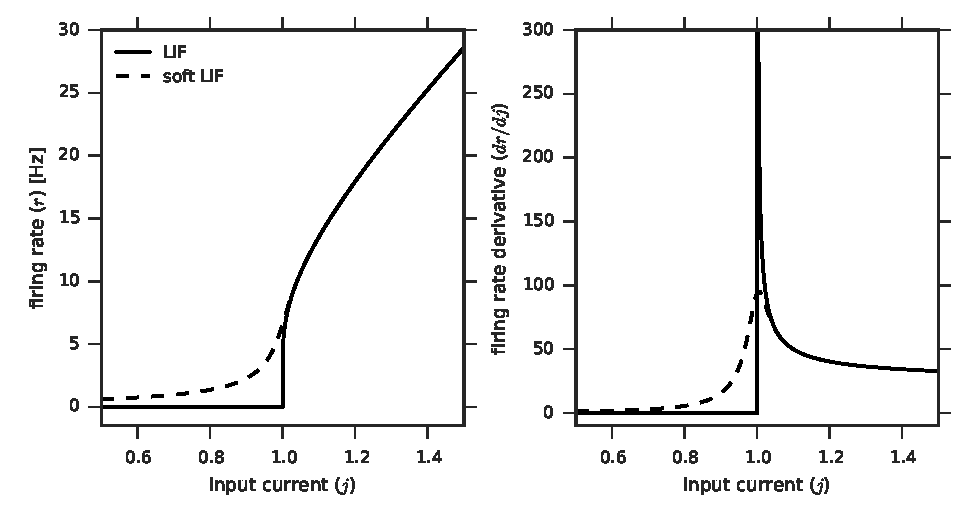
\includegraphics[width=6in]{softlif.pdf}
  \captionb{Comparison of LIF and soft-LIF response functions.}{
    The left panel shows the response functions themselves.
    The LIF function has a hard threshold at $j = V_{th} = 1$;
    the soft-LIF function ($\gamma = 0.01$) smooths this threshold.
    The right panel shows the derivatives of the response functions.
    The hard LIF function has a discontinuous and unbounded derivative
    at $j = 1$; the soft-LIF function has a continuous bounded derivative,
    making it amenable to use in backpropagation.
  }
  \figlabel{softlif}
\end{figure}

By replacing this hard maximum with a softer maximum,
such as $\rho_1(x) = \log(1 + e^x)$,
we can smooth over the hard firing threshold of the LIF neuron.
This smoothed equation is no longer discontinuous in its derivative;
the derivative is bounded.
Further, we can use the substitution
\begin{align}
  \rho_2(x) = \gamma \log\left[1 + e^{x / \gamma}\right]
  \eqnlabel{softrelusigma}
\end{align}
to allow us control over the amount of smoothing,
where $\rho_2(x) \to \max(x, 0)$ as $\gamma \to 0$.
\fig{softlif} compares of the LIF and soft-LIF rate response functions.

By reducing $\gamma$, we can make the soft-LIF rate response function
arbitrarily close to the LIF rate response function,
allowing the soft-LIF function to accurately model
the firing rates of the spiking LIF neurons used during testing.
Of course, having $\gamma$ be too small results in the same
ill-behaved derivative that the soft-LIF model is designed to avoid,
making the choice of $\gamma$ an empirical tradeoff.
In practice,
the precise choice of $\gamma$ does not appear to have
a large effect on network accuracy.
As long as the network does not learn to rely on the small activation
that the soft-LIF neuron has below the LIF neuron firing threshold,
then switching from soft-LIF to LIF neurons will not introduce significant error.
Since a classification network is trying to differentiate between different classes,
it tends to want individual neurons to be selective between classes,
responding strongly in the presence of some classes
and being silent in the presence of others.
This is does not mean that the input driving any particular neuron
is bimodally distributed;
in fact, the input currents across all neurons in a layer
appear unimodally distributed.
Rather, a neuron looking to be strongly and robustly representative of a class
will form strong connections with the strongly and robustly activated neurons
in the previous layer,
since these are the most reliable for classification.
Thus the network will not tend to rely on the weak activations of many neurons,
and the below-threshold activation of the soft-LIF model
should have minimal effect.

This is especially the case when training with noise (\scn{noise-models}).
Noise on the inputs to a neuron is more detrimental
when the neuron is active in an area of its rate-response curve with a large derivative,
since fluctuations in the input will have larger effects on the output.
For the LIF neuron, the rate-response derivative is highest at the firing threshold,
and lowest below the firing threshold (where it is zero)
and well above it (where it approaches zero).
Additionally, filtered spike trains show the most variability
when the firing rate is low (see \fig{lifvariance}).
Both of these factors penalize neuron activities around the firing threshold,
since these result in the most variable outputs.
The result is that neural activations near the firing threshold
should not be relied on by the network,
and switching from soft-LIF to LIF neurons should have little effect.

%% The fact that noise can cause sub-threshold neural firing
%% actually forms the biological motivation for the soft-LIF curve.
The soft-LIF curve has a biological motivation.
High-frequency variability (``noise'') in the membrane voltage of a neuron,
caused for example by random fluctuations in ion-channel opening and closing
\parencite{Manwani1999},
can cause a neuron to fire for a constant input that is slightly below
its firing threshold.
Thus, the response of a LIF neuron model with noise in the membrane voltage
looks qualitatively similar to the soft-LIF response function.
The response of such a noisy LIF neuron
can be modelled using the Siegert approximation
\parencite{Siegert1951,Kreutz-Delgado2015}.
This approximation requires numerically computing an integral
across a complex integrand.
The soft-LIF function provides a similar effect
while being much simpler to implement,
making it more amenable for training networks on GPUs, for example.


\subsection{Modelling spiking variability}
\scnlabel{noise-models}

A key difference between spiking and rate networks
is that spiking networks have much more variability
in the signals passed between neurons.
The output of a spiking neuron (\ie/ a series, or ``train'', of spikes)
is highly variable;
the signal is very large at some points in time (when a neuron spikes),
and zero at all other points in time (between spikes).
Luckily, synapses have an effect of lowpass-filtering these signals (see \scn{synapses}),
reducing the variability.
Still, the variability of the filtered signal is significant.
%% The amount of variability also depends on the firing rate of the neuron
The result is that whereas a rate network will produce a constant output
given a constant input,
a spiking network will have a variable output even for a constant input.
Understanding how the synaptic filter affects a spike train is
the key to understanding variability in spiking networks,
and the first step in reducing its adverse effects.

\begin{figure}
  \centering
  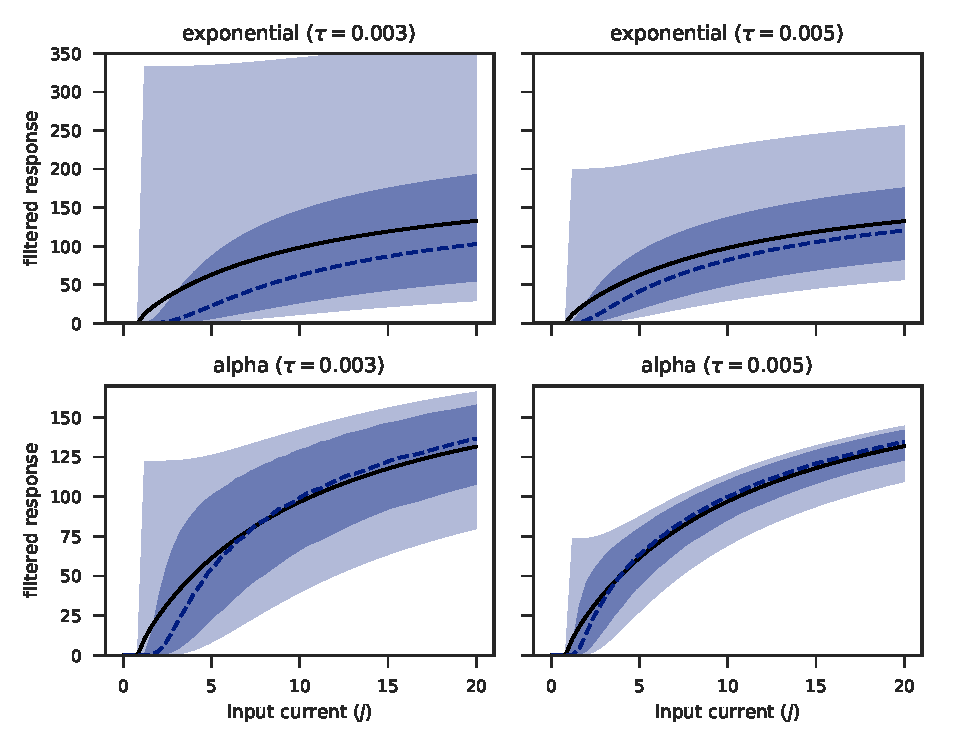
\includegraphics[width=\columnwidth]{lif_variance}
  \captionb{Effect of presynaptic input current on variance of postsynaptic current.}{
    The black line shows the average of the filtered postsynaptic signal
    (which is identical to the average firing rate given by \eqn{lifrate},
    since the filtering is linear).
    The dashed line shows its the median of this signal.
    The darker region indicates the range of its middle quartiles
    (25\sth/ percentile to 75\sth/ percentile).
    The lighter region indicates its full range (minimum to maximum).
  }
  \figlabel{lifvariance}
\end{figure}

\fig{lifvariance} shows the variability of filtered spike trains
across various levels of input current,
for different types of filtering.
Low levels of filtering (\eg/ the exponential filter with $\taus = 0.003$ s)
results in filtered spike trains that are highly variable.
Both increasing the synaptic time constant $\taus$
and increasing the order of the filter from first-order (exponential filter)
to second-order (alpha filter) reduce the amount of variability.
One significant difference between the two synapse models
is that the exponential synapse still has non-zero variance
even for large firing rates,
whereas with the alpha synapse the variance goes to zero
as the firing rate increases
(see \app{spike-model-limits} for a proof).
Due to the significantly lower variance of the alpha synapse,
it will be the main synapse model used in this thesis.

If we can mimic the effects of this spiking variability when training networks,
then ideally the network will become more robust to that variability,
and the resulting networks will run better in spiking neurons
than those trained without noise.
To do this, we need a model that can mimic the variability
in the neuron output given the neuron's firing period $p$.
The first model I experimented with was a simple Gaussian noise model:
\newcommand{\mgauss}{m_\text{G}}
\begin{align}
  \mgauss(p) = \begin{cases}
    \frac{1}{p} + N(0, \sigma) & \text{if } \frac{1}{p} > r_1 \\
    \frac{1}{p}                & \text{otherwise}
  \end{cases} \text{ .}
\end{align}
That is, the noisy output of the neuron is equal to the firing rate
(the inverse of the firing period)
plus additive Gaussian noise with zero mean and standard deviation $\sigma$.
I only add noise if the firing rate is greater than $r_1 = r(j=1)$,
the firing rate of the neuron model at the firing threshold $j = 1$.
The idea behind this is to not add noise when the neuron is silent,
since there is no variability in that case.
The soft-LIF model's firing rate never becomes exactly zero, however,
it only approaches zero as $j \to -\infty$.
I thus chose to add noise only when the input current $j > 1$,
that is, when the corresponding LIF neuron would be firing.
The $\sigma$ parameter can be fit to the empirically-measured
spiking neuron output variance, as characterized in \fig{lifvariance}.
This makes the model amenable to any synapse model.
The main drawbacks to the model are that it models the noise as Gaussian
(which it is not, particularly for low firing rates, see \fig{lifvariance}),
and that it treats the amount of variance as constant across all firing rates
(which again is not the case).

For certain synapse models---including the alpha synapse---%
we can more accurately model the variability of a filtered spike train.
Making the assumption that neurons in the network
are all spiking at constant rates,
we can model the variability in the network
by applying a synaptic filter to a train of spikes at regular intervals,
and looking at the resulting signal.
The result of filtering a spike train with an alpha synapse is given by:
\newcommand{\salpha}{s_\alpha}
\newcommand{\malpha}{m_\alpha}
\begin{align}
  \salpha(t) &= \frac{e^{-t/\taus}}{\taus^2} \left(
    \frac{t}{1 - e^{-p/\taus}} + \frac{p e^{-p/\taus}}{\left(1 - e^{-p/\taus}\right)^2} \right)
  \eqnlabel{alpha-model}
\end{align}
where $\taus$ is the synaptic time constant
and $p$ is the period between spikes.\footnote{
  A full derivation for this equation is given in \app{spike-derivations},
  \eqn{alpha-series}.}

% --- using this noise in real networks is too much variability at lower spike
%   rates. Real networks integrate info over time, less affected by noise.
We can use the alpha-filtered impulse train series
to generate noise in a rate-based network during training,
to help simulate the variability caused by spikes.
To do this, we assume that each input neuron is firing at a constant rate,
and that at any given point in time,
the time since the last spike of the neuron is uncorrelated with all other neurons
(\ie/ firing is completely desynchronized).
To sample from \eqn{alpha-model} for a neuron with firing period $p$,
I generate a random $t \sim U(0, p)$
(that is, $t$ is uniformly distributed between zero and $p$).
Thus, the alpha noise model describes the noisy output of a neuron
with firing period $p$ as $\malpha(p) = \salpha(U(0, p))$.

Despite the fact that \eqn{alpha-model} perfectly models
the filtered output of a regularly-spiking neuron,
it is actually a poor model for spike noise
because it over-estimates the variability in the network due to spikes.
This is because spiking neurons integrate information over time,
helping to smooth out the large fluctuations present in \eqn{alpha-model}.
To account for this, I combined the effects of the synaptic filter
with the filtering effects of the postsynaptic neural membrane.
Applying this combined filter to a spike train results in the following model:
\newcommand{\salphatau}{s_{\alpha\tau}}
\newcommand{\malphatau}{m_{\alpha\tau}}
\begin{align}
  \salphatau(t) &= \frac{\taurc}{d^2}\left(
    \frac{e^{-t/\taurc}}{1 - e^{-p/\taurc}} - \frac{e^{-t/\taus}}{1 - e^{-p/\taus}}\right)
  - \frac{e^{-t/\taus} \left(t (1 - e^{-p/\taus}) + p e^{-p/\taus}\right)}
         {d \taus \left(1 - e^{-p/\taus}\right)^2} \text{ ,}
  \eqnlabel{alpharc-model}
\end{align}
where $d = \taurc - \taus$.
The corresponding noise model is given by $\malphatau(p) = \salphatau(U(0, p))$.

\begin{figure}
  \centering
  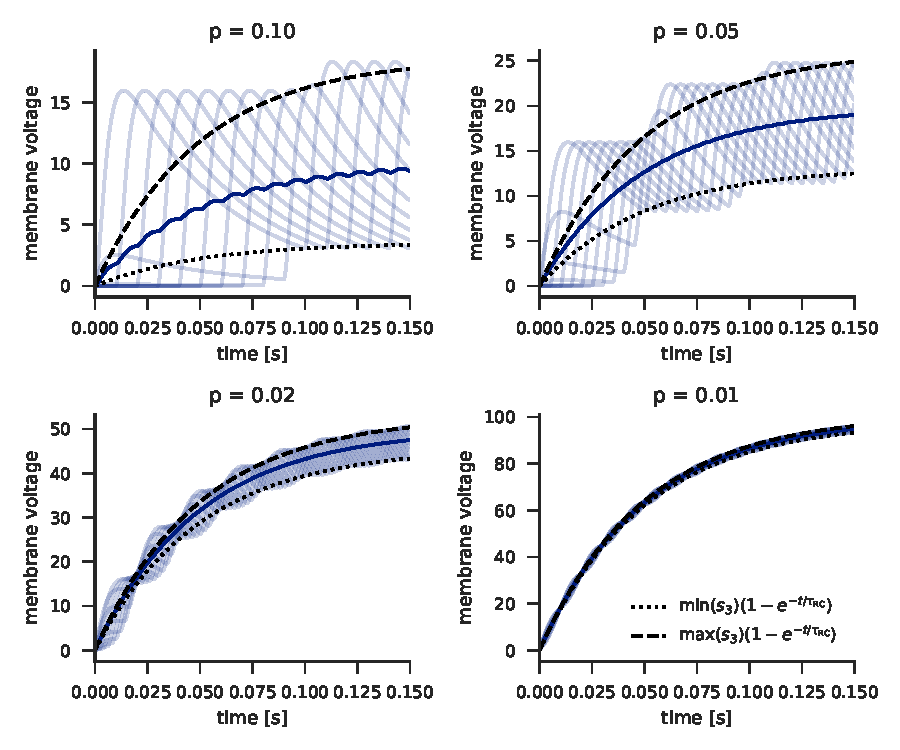
\includegraphics[width=\columnwidth]{alpharc_distribution}
  \captionb{Evaluation of the $\malphatau(t)$ noise model.}{
    To evaluate the $\malphatau(t)$ noise model (\eqn{alpharc-model}),
    I compared voltage traces of a neuron receiving input from an
    alpha-filtered spike train (solid blue traces),
    with an exponential increase to the minimum and maximum of $\salphatau(t)$
    (dotted and dashed traces).
    The light solid traces show individual neuron membrane voltages
    with different input spike train phases (offsets).
    The dark solid trace shows the average of the individual neuron traces.
    Each plot shows a different period $p$ for the input spike train.
    Since the neuron input is not modulated by connection weights,
    the membrane voltage is in arbitrary units.
    $\taurc = 0.05, \taus = 0.003$
  }
  \figlabel{alpharc-minmax}
\end{figure}

To evaluate how well $\salphatau(t)$ actually represents
the variability caused by spikes,
I examined how the range of this series compares to
the actual membrane voltages of an LIF neuron with an
alpha-filtered spike train input at different periods (\fig{alpharc-minmax}).
When we sample from $\salphatau(t)$ to generate a noisy output of a neuron
with spiking period $p$,
we get a value that represents the steady-state of the neuron membrane voltage;
that is, the membrane voltage will exponentially approach this value.
The neuron will spike when its membrane voltage crosses the firing threshold.
Because the connection weights can scale the input arbitrarily,
and scaling all inputs is equivalent to scaling the firing threshold,
we can view the firing threshold as being at any point of the y-axis
in \fig{alpharc-minmax}.
The point in time at which the voltage crosses the firing threshold
determines the firing rate.
The lighter solid lines in \fig{alpharc-minmax} show the membrane voltage
of an LIF neuron subject to an alpha-filtered spike train with period $p$,
given that the neuron has just fired a spike and the voltage is reset to zero.
Each line shows a different phase (\ie/ different temporal offset)
for the filtered input spike train.
The dashed lines show an exponential approach
to the minimum and maximum of $\salphatau(t)$.
These indicate the range of variability that we can get
by using the $\salphatau(t)$ distribution for noise generation in the model.
If we draw a horizontal line through any point in the graph
(corresponding to setting the neuron firing threshold at this value),
the places where the solid lines intersect will represent the range
of possible inter-spike intervals (ISIs) for an actual neuron with spiking input,
and the space between the dashed lines will represent the range
of possible inter-spike intervals using the $\salphatau(t)$ noise model.
If $\salphatau(t)$ represents well the variability caused by spikes,
then these two ranges should correspond well for any horizontal line we draw.
This would mean that wherever the firing threshold of the neuron is
(\ie/ whatever the magnitude of the inputs),
the actual variability caused by spikes will be well represented by the model.

As we see in \fig{alpharc-minmax},
the fit of the noise model depends on both the period of the input spike train
and the amount of time we allow for the membrane voltage to settle.
For all input spike periods $p$,
if we allow the membrane voltage sufficient settling time ($t > 3\taurc$),
then the $\salphatau(t)$ noise model represents the spiking variability well.
This corresponds to the situation when the firing rate of the
output neuron is low.
For higher input spike rates (smaller $p$),
the noise model also does a reasonably good job representing
the spiking variability for $t < 3\taurc$,
as shown in the bottom two panels.
In this situation, the output spike rate can be higher
while still having the variability be well modelled.
As the input spike rates get lower (larger $p$),
the noise model gets progressively worse at capturing
the full range of variability caused by spikes
before the voltage has had time to settle,
as shown by the light solid traces not falling
within the dotted and dashed lines at earlier times.
The worst case scenario is when input spike rates are low,
but the output spike rate is high (\ie/ an ISI of less than $\taurc$).
In this case, the model severely underestimates
the amount of variability caused by spikes.
In practice, this seems to be an uncommon situation,
since the firing rate of neurons
typically decreases from one layer to the next (see \tab{spike-rates}).

\begin{figure}
  \centering
  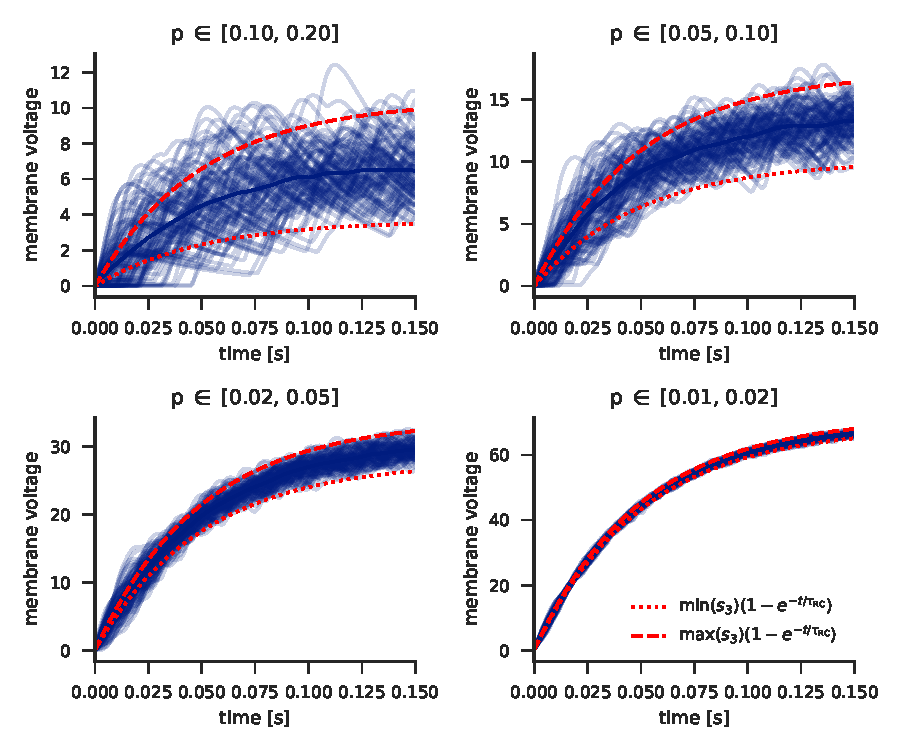
\includegraphics[width=\columnwidth]{alpharc_multiperiod}
  \captionb{Evaluation of the $\malphatau$ noise model with multiple inputs.}{
    Each neuron gets five alpha-filtered spike train inputs,
    with periods $p$ linearly spread across the given ranges (separate panels).
    Each light trace shows one trial (100 trials total),
    where the phases (temporal offsets) of each input are determined randomly.
    The dotted and dashed lines show the minimum and maximum across all trials
    of the noise model,
    where the value of the noise model for one trial is the mean across the
    nine neurons of $\salphatau(t)$ evaluated at the period and offset time for that neuron.
    Since the neuron input is not modulated by connection weights,
    the membrane voltage is in arbitrary units.
    $\taurc = 0.05, \taus = 0.003$
  }
  \figlabel{alpharc-multineuron}
\end{figure}

So far, this analysis has considered the case
when we have a single input neuron,
but in actual networks, each neuron gets input from multiple neurons.
\fig{alpharc-multineuron} looks at this case.
It makes the assumption that we have nine input neurons,
all with the same input weighting and randomly chosen phases,
and with firing periods spread uniformly between two values (distinct for each panel).
This analysis shows similar results as before:
when the membrane voltage is allowed to relax towards its steady state,
the noise model performs well.
For shorter filtering times (\ie/ fast output firing rates)
and for longer input periods,
the model underestimates the variability caused by spikes.
However, the magnitude of these errors is generally smaller,
due to the fact that some of the variability caused by the different inputs
cancels out, assuming the neurons are not synchronized.


\subsection{Training methods}
\scnlabel{spike-training}

To train the network,
I used backpropagation to determine the parameter gradients (\scn{backprop}),
and stochastic gradient descent as an optimization strategy (\scn{sgd}).
This is the same method used by \textcite{Krizhevsky2012},
and is common for training deep neural networks.

For the most part,
the architectural modifications described in \scn{spike-architecture}
had little effect on the training procedure.
One exception is that the parameters used for the LIF neurons---%
namely the bias, gain, amplitude, $\taurc$, $\tref$, and $\gamma$---%
had a large effect on the success of the training.
The most important factor when choosing all of these parameters
is that for the initial weights and biases in the network,
the derivatives of the nonlinearities for inputs from the dataset
should be around one.
This helps to discourage both the vanishing gradient problem
(where the gradient in the lower layers becomes too small),
and the exploding gradient problem
(where the gradient becomes too large).
For ReLU nonlinearities, this is easy,
since the derivative of a ReLU is one whenever it is active.
This is one characteristic that makes training networks with ReLUs much easier,
but it is not the case with the LIF (or soft-LIF) nonlinearity.
By default, the firing threshold of a LIF neuron corresponds to $J = 1$,
so the first change that I made is to give it a bias of one
such that the firing threshold is at zero.
Second, I chose the membrane time constant ($\taurc$) of the neurons.
Smaller values ($\taurc = 0.02$) caused problems with training,
so I chose $\taurc = 0.05$,
which makes a smoother transition between the silent and spiking regimes
of the neuron, and thus a less extreme gradient.
It is possible that shorter $\taurc$ can be used
if other parameters---such as the magnitudes of the initial weights---%
are more judiciously chosen.
I chose $\tref = 0.001$ to be small,
to reduce the effects of saturation on neuron behaviour.
I found that $\gamma$---the amount of smoothing for the ``soft'' LIF---%
could actually be quite small and still train successfully;
I chose $\gamma = 0.02$.
Smaller $\gamma$ is desirable because it makes the soft-LIF curve
closer to the LIF curve,
thus creating less error when switching to spiking neurons.
Finally, I chose the neuron gain and amplitude
(that is, multiplicative scaling on the input and output, respectively)
such that the soft-LIF curve fit the ReLU curve as closely as possible
for inputs in the range $[-1, 10]$.
This ensures that both the magnitude of the soft-LIF output
is in a reasonable range,
and that the soft-LIF derivative has a maximum around one.

The ImageNet (ILSVRC-2012) dataset required one additional modification:
initial pretraining over a few ($\sim$30) batches using a small learning rate,
to bring the initial parameters into a more reasonable range.
Otherwise, beginning with a normal learning rate
would lead to instability in the training.


\subsection{Evaluation methods}
\scnlabel{spike-evaluation}

When evaluating the network,
all off the rate-based (soft-LIF) neurons are replaced with spiking LIF neurons,
and the network is run online.
The spiking classification procedure is the same as in the previous chapter
(see \scn{nef-spiking-methods}).
As with those networks,
the amount of time required to get a reasonable classification result
is an empirical question,
depending on the synaptic time constant $\taus$
and how small we wish to make the margin of error between the spiking network
and its ANN counterpart;
I examine this in \scn{spike-efficiency}.

% no multiview testing
One key difference with \textcite{Krizhevsky2012}
is that they used multiview testing:
many (9) different image patches (chosen in a $3 \times 3$ grid covering the image)
are all passed through the classifier,
and the final classification is determined by averaging the softmax outputs
across all views,
and taking the class with the highest average.
Presenting multiple views requires multiple passes through the network,
which is not realistic for a spiking network.
Each view could be presented sequentially,
but this would take significantly more processing time.
I also experimented with jittering the input image over time
to simulate the effect of multiple views in a shorter time scale;
this did not lead to better classification results.

These models were run using the Nengo simulator \parencite{Bekolay2014}.
In particular, the Nengo OCL backend\footnote{
  \url{https://github.com/nengo/nengo_ocl}}
was used to run the networks efficiently on a GPU.
I made significant additions to the backend
specifically for running convolutional networks efficiently.

%% Another key difference with some other works is that here,
%% each stimulus is presented in series without resetting the network
%% in between presentations \parencite[\cf/][]{Cao2014,Diehl2015}.
%% Each stimulus is also only presented once,
%% which differs from \textcite{Diehl2015} who present each stimulus
%% five times and average over


\section{Results}
\scnlabel{spike-results}

This section provides results from training and running
the spiking network on the datasets described in \scn{datasets}.
The experiments comparing the effects of noise on network training and testing
are performed on the CIFAR-10 dataset,
since it is sufficiently small to allow training many networks (for robust results).


\subsection{System overview}

\begin{figure}
  \centering
  %% 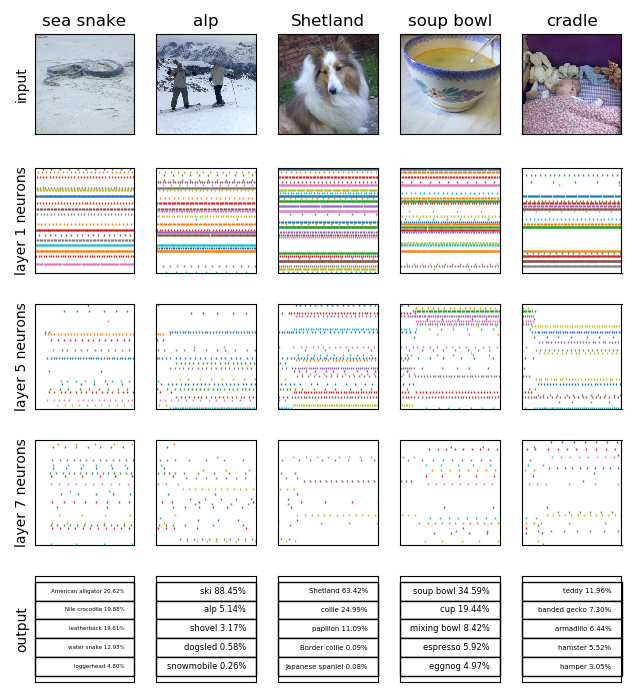
\includegraphics[width=5.8in]{imagenet_demo.png}
  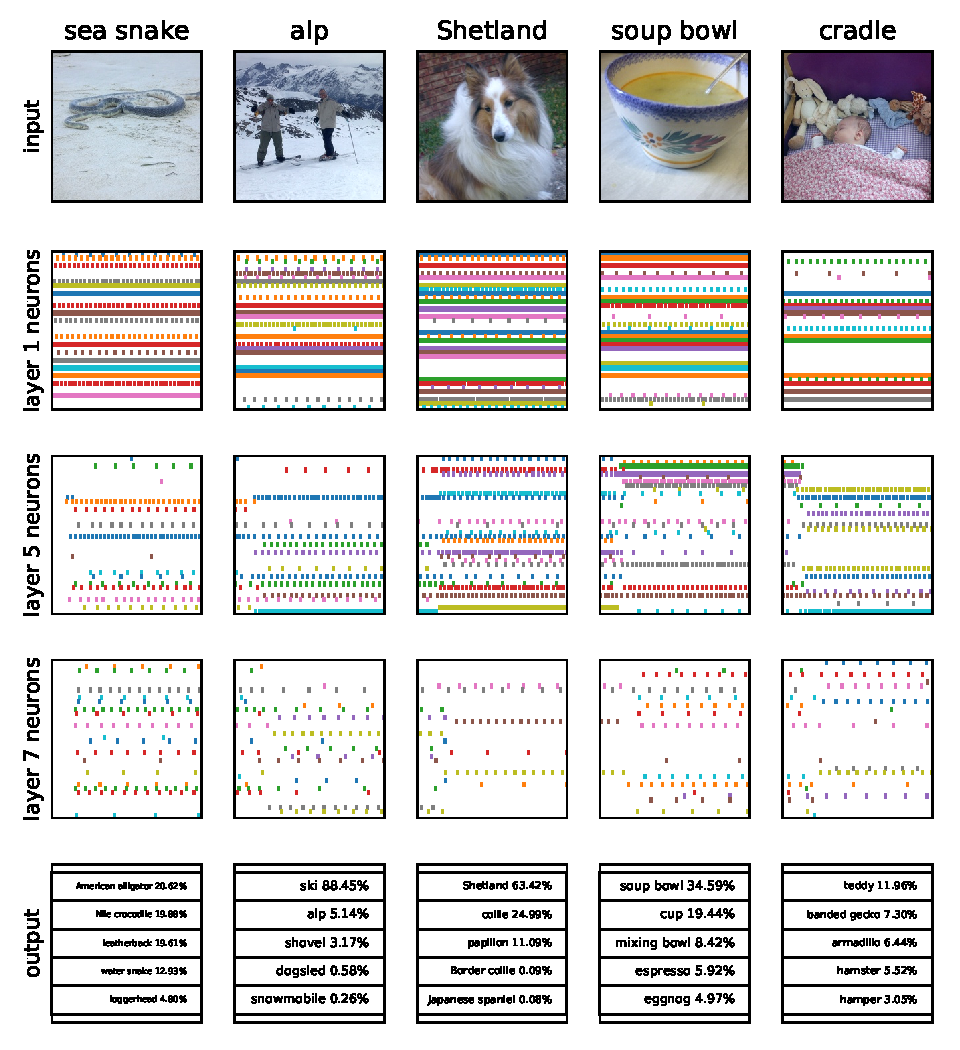
\includegraphics[height=6.4in]{imagenet_demo.pdf}
  \captionb{The spiking system running on several ImageNet images.}{
    Images are presented to the network (top row),
    which processes them using seven layers of spiking neurons (middle three rows).
    The activities in the final spiking layer are decoded to
    probabilities of membership in each of the 1000 possible classes
    (the five most probable classes are shown).
    A video demonstration is available at \url{https://youtu.be/VWUhCzUDZ70}.
  }
  \figlabel{imagenet-demo}
\end{figure}

\fig{imagenet-demo} provides an overview of the system
running on ImageNet test images.
As images are presented sequentially to the network (top row),
they result in spiking activity through the various layers in the network
(middle rows).
The output of the system is weightings on all of the object categories,
which can be used to assign probabilities and predict the class of the image
(bottom row).
The synapses between subsequent layers in the network,
as well as the neural dynamics themselves,
both contribute to delays between successive layers.
Most of the first layer neurons respond almost instantaneously
to a change in the input stimulus,
but later layers take longer to transition to the new activity regime.
The model is often able to correctly predict the object class,
either as its first guess (see ``Shetland'' and ``soup bowl'')
or in its top five guesses (see ``alp'').
Even when the model is not correct, it is often in the right ballpark,
guessing similar objects (see ``sea snake'').
Sometimes, the model is wildly incorrect,
as in the case of ``cradle'' when it guesses ``banded gecko'',
``armadillo'' and ``hamster''
(though the first guess, ``teddy'', is accurate).
These images also illustrate the difficulty of the ImageNet dataset,
which is why researchers typically focus on having the correct category
in the top five guesses of the system,
rather than requiring the system to guess the correct class outright.


\subsection{Architecture modifications and noise}

This section examines the effects of different modifications
to the architecture on the CIFAR-10 dataset.
The starting point is a network trained as per \textcite{Krizhevsky2012}.
The measured test-set error (14.03\%) is considerably higher than
the number reported by \textcite{Krizhevsky2012} ($\sim$11\%),
mainly because the version presented here does not use multiview testing,
whereas the original work does (see \scn{spike-evaluation}).

\begin{table}
  \begin{minipage}{\columnwidth}
  \centering
  \begin{tabular}{llr}
    \# & Modification & CIFAR-10 error \\\hline\hline
    0 & Original ANN \footcite[Based on][]{Krizhevsky2012} & 14.03\% \\
    1 & Network 0 minus normalization & 14.38\% \\
    2 & Network 1 with average-pooling & 16.70\% \\\hline
    3 & Network 2 with soft-LIF & 15.89\% \\  % cifar10-lif-1589
    4 & Network 3 with training noise ($\sigma = 10$) & 16.01\% \\  % cifar10-lif-1628
    5 & Network 3 with training noise ($\sigma = 20$) & 16.92\% \\\hline  % ?
    6 & Network 3 ($\sigma = 0$) in spiking neurons & 17.01\% \\
    7 & Network 4 ($\sigma = 10$) in spiking neurons & \textbf{16.46\%} \\
    8 & Network 5 ($\sigma = 20$) in spiking neurons & 17.04\% \\
  \end{tabular}
  \end{minipage}
  %% \vspace{0.2em}
  \captionb{Effects of successive architectural modifications to CIFAR-10 error.}{
    We first show the original ANN based on \textcite{Krizhevsky2012},
    and then the effects of each subsequent modification.
    Rows 6-8 show the results of running ANNs 3-5 in spiking neurons, respectively.
    Row 7 is the best spiking network, using a moderate amount of training noise.
    While these values provide a rough qualitative characterization
    of the effects of the architectural modifications,
    each error measurement only represents one network trained
    with a particular set of hyperparameters.
    A more robust analysis of the effects of training with noise
    is presented in the next section.
  }
  \tablabel{archmods}
\end{table}

The full list of modifications and the associated error measurements
are shown in \tab{archmods}.
The first modification (Network 1) removes the cross-map response normalization layers,
which only affects the test-set accuracy slightly ($\sim 0.3\%$).
The second modification (Network 2) replaces max-pooling with average-pooling,
which is more detrimental to the accuracy ($\sim 2.3\%$).

Network 3 introduces soft-LIF neurons.
This network is now a rate-based version of the final spiking network,
and thus serves as a baseline for the performance of later networks.
Surprisingly, the error rate of Network 3 is lower than that of Network 2,
that is, introducing soft-LIF neurons increases the accuracy of the network (by $\sim 0.8\%$).
However, this result is not necessarily significant.
Network accuracy depends heavily on the hyperparameters used \parencite{Bergstra2012},
and even slightly on the random initial values chosen for the learned parameters.
Thus, without extensive hyperparameter optimization,
we cannot draw the conclusion that the soft-LIF neuron is better than ReLUs,
even for this particular network.

Network 6 shows Network 3 run in spiking neurons.
I also trained two networks with moderate (Network 4) and high (Network 5)
amounts of Gaussian noise on the neuron firing rates,
and ran these networks in spiking neurons (Networks 7 and 8).
As shown by Networks 4 and 5,
training with even moderate noise reduces the accuracy of the network
(by $\sim 0.1\%$, not necessarily significant),
with more noise being more detrimental to performance ($\sim 1.0\%$).
However, when running in spiking neurons,
the network trained with a moderate amount of noise performs the best
(by $\sim 0.5\%$).
This demonstrates that the right amount of training noise
is able to make the network somewhat robust to the variability that
comes with running the network in spiking neurons.
This result is explored more robustly in the following section.


\subsection{Performance of noise models}
\scnlabel{spike-noise-results}

The previous section demonstrated that adding noise (with the Gaussian model)
can help to reduce the error in spiking networks.
To more robustly assess the benefits of training with noise,
I trained multiple (5) models on CIFAR-10 using the Gaussian noise model
with two different levels of noise,
as well as the models developed in \scn{noise-models},
specifically $\salpha$ (\eqn{alpha-model}) and $\salphatau$ (\eqn{alpharc-model}).
The results are shown in \tab{cifar10-noisemodels}.

\begin{table}
  \centering
  \begin{tabular}{lrrrrr}
    Noise model &
    \multicolumn{1}{c}{ANN} &
    \multicolumn{1}{c}{Spiking 1} &
    \multicolumn{1}{c}{Spiking 2} &
    \multicolumn{1}{c}{Spiking 3} &
    \multicolumn{1}{c}{Spiking 4} \\\hline
None &
15.57 (0.19) & 17.86 (0.30) & 16.99 (0.35) & 16.38 (0.19) & 16.31 (0.26) \\
$\mgauss$ ($\sigma = 10$) &
16.03 (0.12) & 17.15 (0.09) & 16.68 (0.22) & 16.38 (0.08) & 16.40 (0.13) \\
$\mgauss$ ($\sigma = 20$) &
16.96 (0.14) & 17.44 (0.24) & 17.29 (0.12) & 17.37 (0.12) & 17.43 (0.15) \\
$\malpha$ ($\taus = 3$ ms) &
18.49 (0.22) & 18.66 (0.24) & 18.48 (0.18) & 18.72 (0.28) & 18.68 (0.26) \\
$\malpha$ ($\taus = 5$ ms) &
16.96 (0.19) & 17.42 (0.32) & 17.22 (0.12) & 17.13 (0.20) & 17.20 (0.21) \\
$\malphatau$ ($\taus = 3$ ms) &
15.65 (0.30) & 17.31 (0.26) & 16.55 (0.27) & 16.18 (0.23) & 16.18 (0.25) \\
$\malphatau$ ($\taus = 5$ ms) &
15.66 (0.17) & 17.58 (0.34) & 16.90 (0.26) & 16.38 (0.20) & 16.37 (0.17) \\
  \end{tabular}
  \vspace{0.2em}
  \captionb{CIFAR-10 results from spiking networks trained with different noise models.}{
    Results are the average over five independent networks;
    the standard deviation is shown in parentheses.
    The columns show results for the non-spiking ANN,
    and spiking results using alpha synapses with:
    1) $\taus = 0$ ms, $t_c = 10 ms$, $t_p = 60 ms$;
    2) $\taus = 0$ ms, $t_c = 10 ms$, $t_p = 80 ms$;
    3) $\taus = 3$ ms, $t_c = 60 ms$, $t_p = 150 ms$;
    4) $\taus = 5$ ms, $t_c = 100 ms$, $t_p = 200 ms$.
    Noise, in the right amounts, is able to improve spiking performance,
    particularly in cases where the synapse time constant $\taus$
    used at runtime is small or zero,
    and the amount of time used for classification ($t_p$ minus $t_c$) is short.
    Note that for noise models that use a synapse time constant $\taus$,
    the value of $\taus$ used during training
    (presented with the noise model in the left-most column)
    does not necessarily match the value of $\taus$ used at runtime
    (which varies between the four spiking configurations).
  }
  \tablabel{cifar10-noisemodels}
\end{table}

The most salient result is that training with noise
is most beneficial for spiking networks
when the synapse time constant $\taus$ is small or zero
and the amount of time used for classification is short.
When training the ANN, the noise from the $\malphatau$ model has little effect
on the ANN performance,
whereas noise from the other models (which is generally larger in magnitude)
has on average an adverse effect on ANN performance.
In the first two spiking conditions, when no synapse is used ($\taus = 0$ ms),
the benefits of training with noise are most apparent:
networks trained with the $\malphatau$ model with $\taus = 3$ ms
perform significantly better than networks trained without noise.
The Gaussian noise model with $\sigma = 10$ also performs well in these cases.
When the synapse time constant is longer (3 ms or 5 ms),
the networks trained with either the $\malphatau$ model with $\taus = 3$
or the Gaussian noise model with $\sigma = 10$
perform about as well on average as the networks trained without noise.

The $\malphatau$ model with $\taus = 5$ ms performs closer to the no noise model case;
the higher level of filtering associated with this model
results in only a small amount of noise being added,
and it appears the reduced noise is not enough to significantly affect training.
The $\malpha$ noise model, on the other hand, generally introduces too much noise,
performing considerably worse then the other models across almost all cases;
the same is true of the Gaussian noise model with high noise ($\sigma = 20$).
The exception is when there is no synapse and short classification time (case 1),
when some of the higher-noise models are competitive.


\subsection{Accuracy on various datasets}
\scnlabel{spike-accuracy}

To better quantify the performance of my method of constructing spiking deep networks,
I measured its performance on five datasets,
and compared the results with other state-of-the-art spiking networks.
I used the MNIST, SVHN, CIFAR-10, CIFAR-100, and ImageNet datasets,
described in detail in \scn{datasets}.

A summary of the best test-set error scores are shown in \tab{spike-results}.
On all datasets, the network of spiking LIF neurons (LIF SNN)
is able to achieve results close to that of the non-spiking ReLU network (ReLU ANN).
This both shows that loss is minimal
when going from ReLUs to rate LIF neurons,\footnote{
  The CIFAR-100 dataset shows a considerable increase in performance
  when using soft-LIF neurons versus ReLUs in the ANN.
  However this may not be significant;
  it could simply be due to the training hyperparameters chosen,
  since these were not optimized in any way.}
and that loss is minimal when going from rate LIF neurons to spiking LIF neurons.\footnote{
  The ILSVRC-2012 dataset actually shows a marginal increase in accuracy
  when switching to spiking neurons.
  This is likely not statistically significant,
  and could be because the spiking LIF neurons have harder firing thresholds
  than their soft-LIF rate counterparts.}

\begin{table}
  \centering
  \begin{minipage}{\columnwidth}
    %% \begin{center}
    %% \begin{tabular}{|l|r|r|r|}\hline
    %%   Dataset & ReLU ANN & LIF ANN & \textbf{LIF SNN} \\\hline\hline
    %%   MNIST & 0.79\% & 0.84\% & 0.88\% \\\hline
    %%   SVHN & 5.65\% & 5.79\% & 6.08\% \\\hline
    %%   CIFAR-10 & 16.48\% & 16.28\% & 16.46\% \\\hline
    %%   CIFAR-100 & 50.05\% & 44.35\% & 44.87\% \\\hline
    %%   ILSVRC-2012 & 45.4\% (20.9\%)$^a$ & 48.3\% (24.1\%)$^a$ & 48.2\% (23.8\%)$^a$\\\hline
    %% \end{tabular}
    %% \end{center}
    %% \vspace{-0.2em}
    %% \hspace{5em}$^a$ Results from the first 3072-image test batch.
    \begin{center}
    \begin{tabular}{lrrrrr}
      Network  & MNIST & SVHN & CIFAR-10 & CIFAR-100 & ILSVRC-2012\footnote{
        Results from the first 3072-image test batch.}\\\hline
      ReLU ANN & 0.79 & 5.65 & 16.48 & 50.05 & 45.4 (20.9) \\
      LIF ANN  & 0.84 & 5.79 & 16.28 & 44.35 & 48.3 (24.1) \\
      LIF SNN  & 0.88 & 6.08 & 16.46 & 44.87 & 48.2 (23.8) \\
    \end{tabular}
    \end{center}
  \end{minipage}
  \captionb{Test-set error rates (percent) for spiking LIF networks (LIF SNN).}{
    Compared with ReLU ANN and LIF ANN (both using the same network structure,
    but with ReLU and LIF rate neurons respectively).
    The spiking versions of each network perform
    almost as well as the rate-based versions.
    The ILSVRC-2012 (ImageNet) results show the error for the top result,
    with the top-5 result in brackets.
  }
  \tablabel{spike-results}
\end{table}

\begin{table}
  \centering
  \begin{minipage}{\columnwidth}
    \begin{center}
    \newcommand{\cmpesser}{\label{cmpesser}\textcite{Esser2016}}
    \newcommand{\cmpbatch}{\label{cmpbatch}Results from the first 3072-image test batch.}
    \begin{tabular}{lrrrrr}
      Dataset & \textbf{My model} &
        TN 1-chip\footnote{\cmpesser} &
        TN 8-chip\footnoteref{cmpesser} &
        Zambrano\footcite{Zambrano2017} &
        Best Other \\\hline
      MNIST       & 0.88 (27k) &           &           & 0.44 (100k) & 0.88 (22k) \footcite{Diehl2015} \\
      SVHN        & 6.08 (27k) & 3.34 (1M) & 2.54 (8M) &      & \\
      CIFAR-10    & 16.46 (50k) & 16.59 (1M) & 10.68 (8M) & 10.14 (270k) & 22.57 (28k) \footcite{Cao2014} \\
      CIFAR-100   & 44.87 (50k) & 44.36 (1M) & 34.52 (8M) & 35.79 (295k) & \\
      ILSVRC-2012 & 48.2\footnote{\cmpbatch} (493k) & & & 37.03 (24M) & \\
    \end{tabular}
    \end{center}
  \end{minipage}
  \captionb{Percentage error rates of my model compared with state-of-the-art models.}{
    I compare with recent results on the TrueNorth (TN) neuromorphic chip \parencite{Esser2016},
    as well as other best results in the literature.
    Approximate numbers of neurons are shown in parentheses.
    The TrueNorth networks use significantly more neurons than my networks
    (about 20$\times$ more for the 1-chip network
    and 160$\times$ more for the 8-chip network).
    The ILSVRC-2012 (ImageNet) numbers indicate the error for the top result
    (the top-5 result for this work can be found in \tab{spike-results},
    and was not reported for Zambrano).
    It is important to note that my error on ILSVRC-2012 is only computed
    using the first 3072-image test batch (to reduce computation time),
    and thus only provides an estimate of the true error
    and is not directly comparable to the other result on this dataset.
  }
  \tablabel{spike-comparison}
\end{table}


\tab{spike-comparison} compares my results
with several other state-of-the-art results for deep spiking networks.
A recent paper using the TrueNorth neuromorphic chip \parencite{Esser2016}
set many new records for spiking networks
on the SVHN, CIFAR-10, and CIFAR-100 datasets.
However, these networks use large numbers of neurons,
either one million for the one-chip networks
or eight million for the eight-chip networks.
By comparison, my networks---%
which use orders of magnitude fewer neurons (27-50 thousand)---%
outperform the one-million-neuron TrueNorth networks
on two of the three tasks.
Furthermore, I demonstrate that my methods can perform reasonably well
on the very large ImageNet (ILSVRC-2012) dataset using half a million neurons.
The methods used by \textcite{Esser2016}
would have difficulty scaling a problem of this size due to the sheer
number of neurons required.


\begin{table}
  \centering
  \begin{minipage}{\columnwidth}
    \begin{center}
      \newcommand{\ratbatch}{\label{ratbatch}Results from the first 3072-image test batch.}
      \newcommand{\hunsa}{\textbf{My model}}
      \newcommand{\hunsb}{\hunsa}
      \newcommand{\zamba}{Zambrano\footnote{\label{zamba}\textcite{Zambrano2017}}}
      \newcommand{\zambb}{Zambrano\footnoteref{zamba}}
      \begin{tabular}{llrrrrr}
        Dataset & Method & Error & Neurons & Rate & Time & Spikes/image \\
        \hline\multirow{3}{*}{MNIST}
            & \hunsa & 0.88 & 27.1 k & 9.7 & 200 & 52 k \\
            & \zamba & 0.44 & 100.7 k & 67 & 291 & 1963 k \\
            & \zambb & 0.88 & 100.7 k & 10 & 209 & 210 k \\
        \hline\multirow{3}{*}{CIFAR-10}
            & \hunsb & 16.5 & 49.5 k & 148 & 200 & 1.5 M \\
            & \zambb & 10.1 & 270.8 k & 68 & 372 & 6.9 M \\
            & \zambb & 11.5 & 270.8 k & 22 & 304 & 1.8 M \\
        \hline\multirow{3}{*}{Imagenet}
            & \hunsb & 48.2\footnote{\ratbatch} & 493.2 k & 93 & 200 & 9.2 M \\
            & \zambb & 37.0 & 24085 k & 66 & 347 & 551.6 M \\
            & \zambb & 46.2 & 24085 k & 12 & 338 & 97.7 M
      \end{tabular}
    \end{center}
  \end{minipage}
  \captionb{Comparison of spikes required to classify an image.}{
    Comparing my method with another state-of-the-art method
    (the only method from \tab{spike-comparison} to report overall network firing rates).
    Despite higher firing rates,
    my model uses fewer spikes to classify each image,
    due to the significantly fewer neurons used.
  }
  \tablabel{spike-sota-rates}
\end{table}

It is only quite recently that other another spiking network
has been able to compete on ILSVRC-2012,
namely that of \textcite{Zambrano2017}.
Their networks also use lower firing rates than other state-of-the-art networks
(including the ones presented in this thesis).
However, their networks also use significantly more neurons
than those presented in this thesis.
The result is that the number of spikes required to classify each image
is actually higher than all the networks presented in this thesis
(see \tab{spike-sota-rates}).


\subsection{Efficiency}
\scnlabel{spike-efficiency}

\newcommand{\Esnn}{E_\text{SNN}}
\newcommand{\Esynop}{E_\text{synop}}
\newcommand{\Eupdate}{E_\text{update}}

Running on standard hardware,
spiking networks are considerably less efficient
than their ANN counterparts.
This is because ANNs are static,
requiring only one forward-pass through the network to compute the output,
whereas SNNs are dynamic,
requiring the input to be presented for a number of time steps
and thus a number of forward passes.
On hardware that can take full advantage of the sparsity that spikes provide---%
such as most neuromorphic hardware---%
SNNs can be more efficient than the equivalent ANNs, as we show here.

First, we need to compute the computational efficiency of the original network,
specifically the number of floating-point operations (FLOPs) required to pass
one image through the network.
The two main computations in a spiking neural network
are those associated with the neurons,
and those associated with the connections:
\begin{align}
  \text{FLOPs} &= \frac{\text{FLOPs}}{\text{neuron}} \times \text{neurons} +
                  \frac{\text{FLOPs}}{\text{connection}} \times \text{connections} \text{ .}
\end{align}
Since a rectified linear unit is a simple max function,
it requires only one FLOP to compute ($\text{FLOPs/neuron} = 1$).
Each connection requires two FLOPs, a multiply and an add ($\text{FLOPs/connection} = 2$).
We can determine the number of connections by ``unrolling'' each convolution,
so that the layer is in the same form as a locally connected layer.
(See \tab{network-sizes} for the number of FLOPs
needed to process a single image on conventional hardware
for each different network architecture.)

\begin{table}
  \centering
  \begin{tabular}{r|rrr|rrr|rrr}
    &
    \multicolumn{3}{c|}{MNIST} &
    \multicolumn{3}{c|}{CIFAR-10} &
    \multicolumn{3}{c}{ILSVRC-2012} \\
    Layer
      &  $N$  & $S$  &  $R$ &  $N$  & $S$  & $R$ & $N$  & $S$  & $R$  \\\hline
    0 &       & 314k &      &       & 2.8M &     &      &  70M &      \\
    1 & 12.5k & 5.0M &  4.6 &   37k &  15M & 173 & 194k & 224M & 178  \\
    2 & 12.5k & 6.3M & 15.6 &  9.2k & 1.3M &  99 & 140k & 112M & 48.8 \\
    3 &    2k &  20k &  4.2 &  2.3k & 664k & 9.7 &  65k & 150M & 26.6 \\
    4 &       &      &      &  1.2k &  12k & 7.2 &  43k & 100M & 30.6 \\
    5 &       &      &      &       &      &     &  43k &  38M & 35.6 \\
    6 &       &      &      &       &      &     & 4.1k &  17M & 19.1 \\
    7 &       &      &      &       &      &     & 4.1k & 4.1M & 10.7 \\
  \end{tabular}
  \captionb{Spike rates by layer for my networks.}{
    The number of neurons $N$, synapses out of the layer $S$, and average spike rate $R$ in Hz
    for each layer of each network (k = thousands, M = millions).
    Layer 0 indicates the input layer, which has no neurons,
    so only the synapses out are shown (connecting to the first hidden layer).
    The output layers, which also have no neurons, are not shown.
  }
  \tablabel{spike-rates}
\end{table}

To compute the SNN efficiency on a prospective neuromorphic chip,
we begin by identifying the energy cost
of a synaptic event ($\Esynop$) and neuron update ($\Eupdate$),
relative to standard hardware.
In consultation with neuromorphic experts,
and examining current reports of neuromorphic chips \parencite[\eg/][]{Merolla2014}),
we assume that
each neuron update takes as much energy as 0.25 FLOPs ($\Eupdate = 0.25$),
and each synaptic event takes as much energy as 0.08 FLOPs ($\Esynop = 0.08$).
(These numbers could potentially be much lower for analog chips, \textcite[\eg/][]{Benjamin2014}.)
Then, the total energy used by an SNN to classify one image is
(in units of the energy required by one FLOP on standard hardware):
\begin{align}
  \Esnn = \left(\Esynop \frac{\text{synops}}{\text{s}} +
            \Eupdate \frac{\text{updates}}{\text{s}}\right) \times
            \frac{\text{s}}{\text{image}} \text{ .}
  \eqnlabel{esnn}
\end{align}
These numbers are computed from the per-layer parameters
shown in \tab{spike-rates}:
\begin{align}
  \frac{\text{synops}}{\text{s}} &= \sum_i^L S_i R_i \nonumber\\
  \frac{\text{updates}}{\text{s}} &= \frac{\text{timesteps}}{\text{s}} \times \sum_i^L N_i \nonumber
  \text{ ,}
\end{align}
where $L$ is the number of layers.\footnote{
  The networks in this thesis update every millisecond,
  resulting in 1000 timesteps/s.}
The CIFAR-10 network has rates of
2.69 billion synops/s and 49.5 million updates/s.
This results in the equivalent energy usage as 45.6 million FLOPs
when each image is presented for 200 ms.
Dividing by the number of FLOPs per image on standard hardware (39.1 million),
we find that the relative efficiency of the CIFAR-10 network is 0.76,
that is, it is somewhat less efficient than the ANN,
if we present the images for 200 ms.

\eqn{esnn} shows that if we are able to lower
the amount of time needed to present each image to the network,
we can lower the energy required to classify the image.
Alternatively, we can lower the number of synaptic events per second
by lowering the firing rates of the neurons.
Lowering the number of neuron updates would have little effect on the
overall energy consumption since the synaptic events require the majority of the energy.

To lower the presentation time required for each input while maintaining accuracy,
we need to decrease the synapse time constant as well,
so that the information is able to propagate through the whole network
in the decreased presentation time.
\tab{efficiency} shows the effect of various alternatives
for the presentation time and synapse time constant
on the accuracy and efficiency of the networks for a number of the datasets.

\begin{table}
  \centering
  \begin{tabular}{lrrrrr}
    Dataset & $\tau_s$ [ms] & $t_c$ [ms] & $t_p$ [ms] & Error & Efficiency \\
    \hline\multirow{4}{*}{CIFAR-10}
      & 5 & 100 & 200 & 16.18\% & 0.76$\times$ \\
      & 3 &  60 & 150 & 16.18\% & 0.98$\times$ \\
      & 0 &  10 &  80 & 16.55\% & 1.64$\times$ \\
      & 0 &  10 &  60 & 17.31\% & 2.04$\times$ \\
    \hline\multirow{4}{*}{MNIST}
      & 5 & 120 & 200 & 0.88\% & 5.94$\times$ \\
      & 2 &  40 & 100 & 0.92\% & 10.24$\times$ \\
      & 2 &  50 &  60 & 1.14\% & 14.42$\times$ \\
      & 0 &  20 &  60 & 3.67\% & 14.42$\times$ \\
    \hline\multirow{3}{*}{ILSVRC-2012}
      & 3 & 140 & 200 & 23.80\% & 1.39$\times$ \\
      & 0 &  30 &  80 & 25.33\% & 2.88$\times$ \\
      & 0 &  30 &  60 & 25.36\% & 3.51$\times$ \\
  \end{tabular}
  \captionb{Estimated efficiency of my networks on neuromorphic hardware.}{
    As compared with traditional hardware.
    For all datasets, there is a tradeoff between accuracy and efficiency,
    but we find many configurations that are significantly more efficient
    while sacrificing little in terms of accuracy.
    $\tau_s$ is the synapse time constant,
    $t_c$ is the start time of the classification,
    $t_p$ is the end time of the classification
    (\ie/ the total presentation time for each image).
  }
  \tablabel{efficiency}
\end{table}

\tab{efficiency} shows that for some datasets
(\ie/ CIFAR-10 and ILSVRC-2012)
the synapses can be completely removed ($\tau_s = 0$ ms)
without sacrificing much accuracy.
Interestingly, this is not the case with the MNIST network,
which requires at least some measure of synapses to function accurately.
We suspect that this is because the MNIST network has much lower firing rates
than the other networks
(average of 9.67 Hz for MNIST, 148 Hz for CIFAR-10, 93.3 Hz for ILSVRC-2012).
This difference in average firing rates is also why the MNIST network is
significantly more efficient than the other networks.

\begin{figure}
  \centering
  \begin{tabular}{cc}
    CIFAR-10 ($\tau_s = 5$ ms) & CIFAR-10 ($\tau_s = 0$ ms) \\
    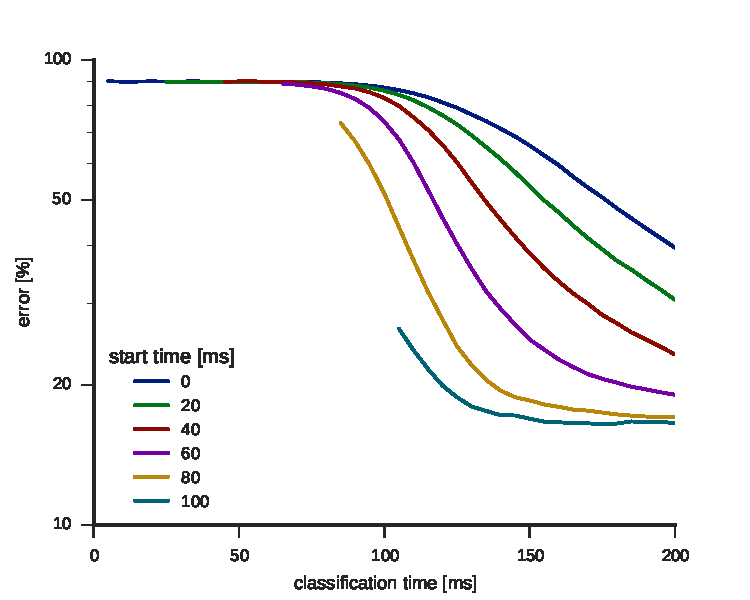
\includegraphics[width=0.4\columnwidth,clip=true,trim=2mm 0mm 10mm 8mm]{cifar10-lif-1628-200ms_pt-classplot.pdf} &
    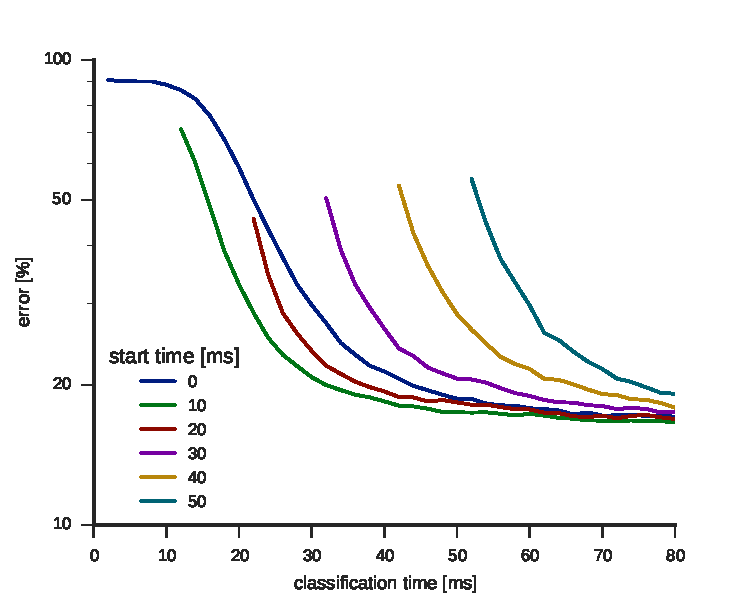
\includegraphics[width=0.4\columnwidth,clip=true,trim=2mm 0mm 10mm 8mm]{cifar10-lif-1628-80ms_pt-0ms_alpha-classplot.pdf} \\
    MNIST ($\tau_s = 2$ ms) & ILSVRC-2012 ($\tau_s = 0$ ms) \\
    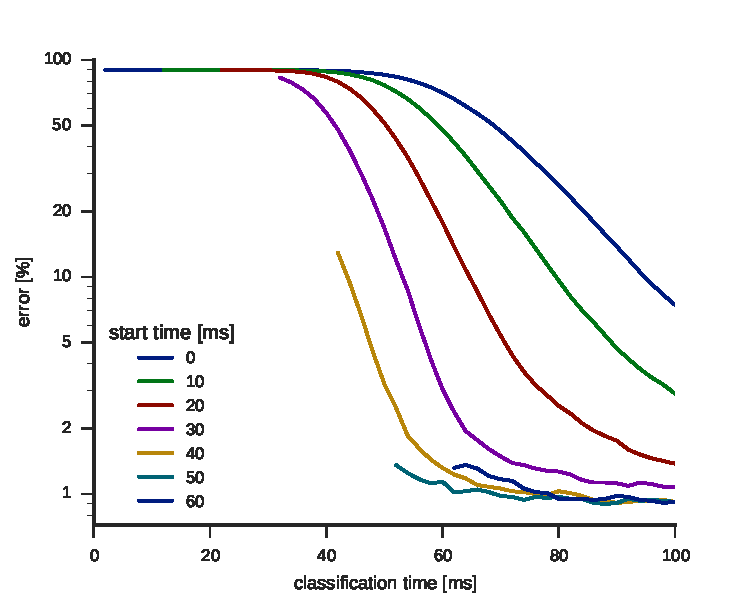
\includegraphics[width=0.4\columnwidth,clip=true,trim=2mm 0mm 10mm 8mm]{mnist-lif-0097-100ms_pt-2ms_alpha-classplot.pdf} &
    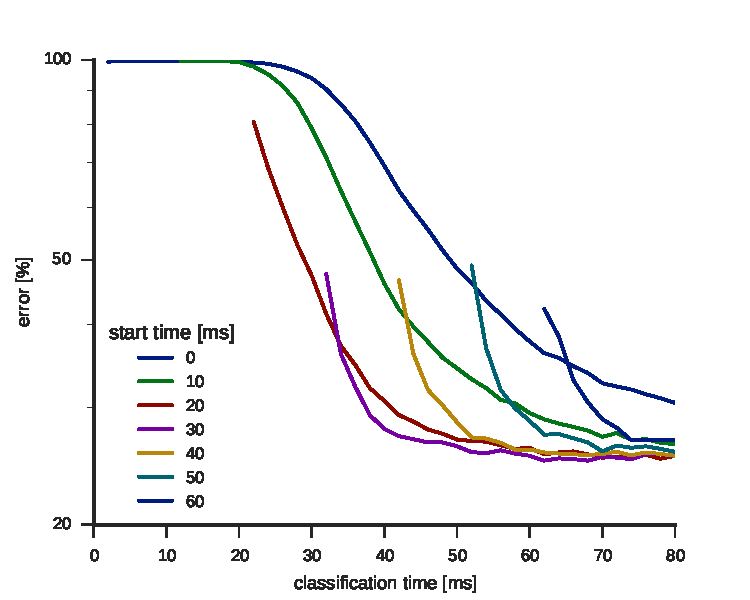
\includegraphics[width=0.4\columnwidth,clip=true,trim=2mm 0mm 10mm 8mm]{ilsvrc2012-lif-48-80ms_pt-0ms_alpha-classplot.pdf} \\
  \end{tabular}
  \captionb{Effects of classification time on accuracy.}{
    Individual traces show different starting classification times ($c_0$),
    and the x-axis the end classification time ($c_1$).
  }
  \figlabel{classtime}
\end{figure}

It is important to tune the classification time,
both in terms of the total length of time each example is shown for ($c_1$),
and when classification begins ($c_0$).
The optimal values for these parameters are very dependent on the network,
both in terms of the number of layers, firing rates, and synapse time constants.
\fig{classtime} shows how the classification time affects accuracy
for various networks.

%% Given that the CIFAR-10 network performs almost as well with no synapses
%% as with synapses,
%% one may question whether noise is required during training at all.
%% We retrained the CIFAR-10 network with no noise and ran with no synapses,
%% but could not achieve accuracy better than 18.06\% in the spiking network.
%% This suggests that noise is still beneficial during training.


\section{Discussion}

The soft-LIF neuron model is able to smooth the LIF rate response function,
such that it is differentiable and usable with backpropagation.
This smoothing technique is also applicable to other neuron models
with a static rate response function and a discontinuity in firing rate
around the firing threshold.
This could include the idiosyncratic neuron models
used on analog neuromorphic hardware \parencite[\eg/][]{Benjamin2014}.

With the soft-LIF model, the amount of smoothing can be adjusted so that
the model is arbitrarily close to the LIF model it is approximating.
This could allow for a relaxation over the course of training
where the soft-LIF model begins quite smooth
and then relaxes towards the actual LIF model,
so that there is no loss when changing to a LIF rate model.
In practice, I have not found that this is necessary.
Optimization tends to push neurons to be either robustly on or off,
particularly when noise is present either on the neural nonlinearity
or in the form of dropout.
This keeps neural inputs away from the firing threshold,
and thus out of the region where the soft-LIF and rate LIF models differ.

% Why does alpha noise model not work? Does not account for neuronal integration
The first noise model I developed for alpha synapses (model $\salpha$, \eqn{alpha-model})
did not perform well.
While this model perfectly characterizes
the variability of an alpha-filtered spike train,
it assumes that downstream neurons only receive an instantaneous snapshot
of the filtered spike train,
when in fact they integrate this spike train over time.
This leaky integration provides a second layer of filtering
on the incoming spike trains,
and is especially significant because the neural membrane time constant $\taurc$
tends to be much larger than the postsynaptic time constant $\taus$.
Without accounting for this filtering,
the model overestimates the amount of noise caused by spiking,
injecting too much noise during training resulting in lower accuracy.
Including the effects of this membrane filtering significantly improves performance.

% Discuss limitations of alpharc noise model
% - already discussed a bit above
% - two factors at play: rate of spikes and amplitude of spikes
%   (as determined by connection weights)
% Can illustrate this with alpharc_empirical.py
When accounting for neuronal integration,
the window over which a neuron is actually able to integrate
depends on its firing rate,
where the integration period is equal to the period between spikes
(minus the refractory period).
For example, a neuron that is firing quickly only integrates its inputs
for a short amount of time before it hits threshold and spikes,
whereas a neuron with a low firing rate
will require much more time to integrate before hitting threshold.
This is illustrated in \fig{alpharc-multineuron},
where the model correctly estimates the spiking variance for low
postsynaptic neuron firing rates,
but underestimates the spiking variance at high firing rates.
In the low firing rate case,
there is more time between spikes and thus
the full filtering effect of the membrane is able to be applied to most inputs;
thus the model---which includes the full membrane filter---does a good job.
As the firing rate increases,
the membrane has less time to filter inputs
and the effective filtering is reduced;
the model now overestimates the amount of filtering being applied to inputs,
thus underestimating the amount of variance in the output.

The firing rate of a neuron depends on the strength of its inputs,
which in turn depend on both the firing frequency and synaptic weighting
of each of its afferent neurons.
This dependence on both input frequency and weighting is important:
it means that to fully characterize the variability of a neuron's input signal,
one needs to transmit both these values for each afferent neuron.\footnote{
  This assumes that each of the input neurons is firing at constant rate,
  and that we are not interested in the phase of any neuron's firing.
  If a neuron's rate is variable (\eg/ a bursting neuron)
  then more values would be needed to fully characterize the variability.
  Similarly, if we are interested in neural phases
  (to account for synchrony between neurons),
  again more information would be needed.}
For example, if we only transmit a single value for each neuron
that is equal to its firing rate times synaptic weighting
(as is standard for rate-based networks),
then a downstream neuron cannot tell the difference
between a high-frequency input with a small weighting,
and a low-frequency input with a large weighting.
Yet, these two inputs have very different amounts of variance,
with a filtered high-frequency spike train
having much less variance than a similarly filtered low-frequency one.
The need for both the firing rate and synaptic weight of input neurons
can be seen in the Siegert model
for the rate of a LIF neuron with Poisson inputs \parencite{OConnor2013}:
it requires both values,
multiplying the weights times the rates to characterize the input mean,
and multiplying the squared weights times the rates to characterize the variance.

It is not theoretically difficult to transmit two values during training---%
or even more to characterize higher moments of the variability distribution---%
and the increase in training time would be
roughly proportional to the total number of moments transmitted
(\eg/ using two moments would take twice as computation in the forward pass
as a typical ANN, which uses only the mean).
Incorporating these values into the backwards pass would be more difficult,
since typical objective functions only constrain the mean firing rates
of the output units.
That said, even incorporating higher moments only in the forward pass
could be beneficial,
since these moments can affect the mean
(as seen in the Siegert model).
Current machine learning libraries are not designed to transmit
multiple values in this manner,
and would require significant modification.
Depending on the exact calculation required for the higher moments,
many of the basic computational elements such as convolution and pooling
may be able to be reused to compute the moments.

The alternative to accounting for such moments in a rate-based optimization method
is to simply switch to a spike-based optimization method.
Due to the relationship between first spike time and firing rate,
spike-based and rate-based methods are optimizing very similar quantities.
The main difference is that by accounting for individual spike times,
spike-based methods can better account for the inherent variability due to spikes.
Furthermore, they can exploit synchrony between neuron spike times,
information that is lost when dealing only in firing rates.
However, this ability to optimize the precise spike times of neurons
assumes that all neurons are starting
from the same resting state for each stimulus presentation.
Not surprisingly, all the networks I am aware of
that use spike-based optimization methods
do reset the system between stimulus presentations,
not only during training but also during testing.
If the system is run continuously, without resetting between presentations,
then much of the advantage of spike-based methods will disappear,
and I expect the two types of networks to perform similarly.
However, I am not aware of any such comparison in the literature.
The exception to this would be on dynamic stimuli,
such as those used by \textcite{Huh2017},
where spike times and synchrony over the course of a single stimulus are important.


%%  LocalWords:  DNNs CNNs cnns spikingmethods Gutig SpikeProp Bohte
%%  LocalWords:  LM Mostafa Stromatias ratemethods Carrasco Cao Diehl
%%  LocalWords:  Esser TrueNorth Merolla SVHN RBMs OConnor Siegert th
%%  LocalWords:  Neftci Eliasmith nef erf conv softlif lrrrr lifrate
%%  LocalWords:  lifraterho softrelusigma lifvariance alpharc minmax
%%  LocalWords:  ISI scn multineuron sgd multiview jittering un STDP
%%  LocalWords:  imagenet archmods Bergstra cifar noisemodels lrrrrr
%%  LocalWords:  synop synops esnn classtime Krizhevsky Levenberg OCL
%%  LocalWords:  Marquardt McKennoch Contrastive AlexNet FLOPs Kreutz
%%  LocalWords:  Manwani backprop Bekolay llr SNN essernote Zambrano
%%  LocalWords:  zamba llrrrrr img sota SNNs rrr cmpesser
